\documentclass[a4paper,12pt,italian]{report}

% =====================================================
% PACCHETTI BASE
% =====================================================
\usepackage[italian]{babel}
\usepackage[T1]{fontenc}
\usepackage{graphicx}
\usepackage{float}
\usepackage{tocloft}
\usepackage{booktabs}
\setlength{\cftchapnumwidth}{2.5em}

\usepackage{amsmath}
\usepackage{amsfonts}
\usepackage{amssymb}
\usepackage{amsthm}
\usepackage[hidelinks]{hyperref}

\usepackage{fancyhdr}
\setlength{\headheight}{14.5pt}
\usepackage{titlesec}
\usepackage{tocloft}
\usepackage{listings}
\usepackage{xcolor}
\usepackage{algorithm}
\usepackage{algorithmicx}
\usepackage[noend]{algpseudocode}
\usepackage{amsmath}
\usepackage{listings}
\usepackage{xcolor}

% Definizione linguaggio JSON per listings
\lstdefinelanguage{json}{
    basicstyle=\ttfamily\small,
    numbers=left,
    numberstyle=\tiny\color{gray},
    stepnumber=1,
    numbersep=8pt,
    showstringspaces=false,
    breaklines=true,
    frame=single,
    rulecolor=\color{gray!30},
    backgroundcolor=\color{gray!5},
    string=[s]{"}{"},
    stringstyle=\color{teal},
    comment=[l]{:},
    commentstyle=\color{black},
    morestring=[s]{:\ \"}{"},
    literate=
        *{0}{{{\color{blue}0}}}{1}
         {1}{{{\color{blue}1}}}{1}
         {2}{{{\color{blue}2}}}{1}
         {3}{{{\color{blue}3}}}{1}
         {4}{{{\color{blue}4}}}{1}
         {5}{{{\color{blue}5}}}{1}
         {6}{{{\color{blue}6}}}{1}
         {7}{{{\color{blue}7}}}{1}
         {8}{{{\color{blue}8}}}{1}
         {9}{{{\color{blue}9}}}{1}
         {true}{{\color{orange}true}}{4}
         {false}{{\color{orange}false}}{5}
         {null}{{\color{orange}null}}{4},
}

% =====================================================
% TEMPLATE TOR VERGATA
% (DEVE essere presente nel progetto)
% =====================================================
\usepackage{tesisty}

% =====================================================
% CONFIGURAZIONE ALGORITMI
% =====================================================
\makeatletter
\def\BState{\State\hskip-\ALG@thistlm}
\makeatother

\algdef{SE}[DOWHILE]{Do}{doWhile}{\algorithmicdo}[1]{\algorithmicwhile\ #1}

\algdef{SE}[VARIABLES]{Variables}{EndVariables}
  {\algorithmicvariables}
  {\algorithmicend\ \algorithmicvariables}
\algnewcommand{\algorithmicvariables}{\textbf{global variables}}

\floatname{algorithm}{Algoritmo}

% =====================================================
% CONFIGURAZIONE LISTINGS
% =====================================================
\addto\captionsitalian{
  \renewcommand{\lstlistingname}{Codice}
}
\addto\captionsitalian{
  \renewcommand{\lstlistlistingname}{Elenco dei codici}
}

\lstset{
  basicstyle=\ttfamily\small,
  breaklines=true,
  frame=single,
  numbers=left,
  numberstyle=\tiny,
  keywordstyle=\color{blue},
  commentstyle=\color{gray},
  stringstyle=\color{red}
}

% =====================================================
% AMBIENTI PERSONALIZZATI
% =====================================================
\newtheorem{obs}{Osservazione}[section]
\newenvironment{oss}
    {\begin{obs}\begin{normalfont}}
    {\hfill $\square$ \end{normalfont}\end{obs}}

\newtheorem{pro}{Problema}[chapter]
\newenvironment{prob}
    {\begin{pro}\begin{normalfont}}
    {\hfill $\spadesuit$ \end{normalfont}\end{pro}}

\newtheorem{teor}{Teorema}[section]
\newenvironment{teorema}
    {\begin{teor}\itshape}
    {\end{teor}}

\newtheorem{defn}{Definizione}[section]
\newenvironment{de}
    {\begin{defn}\begin{normalfont}}
    {\hfill $\clubsuit$ \end{normalfont}\end{defn}}

% =====================================================
% NUMERAZIONE
% =====================================================
\numberwithin{equation}{section}
\setcounter{secnumdepth}{3}
\setcounter{tocdepth}{3}

% =====================================================
% INIZIO DOCUMENTO
% =====================================================
\begin{document}

% =====================================================
% FRONTESPIZIO (TESISTY)
% =====================================================
\titoloTesi{Scheduling adattivo carbon-aware in ambienti serverless: gestione del trade-off energia-accuratezza tramite varianti di funzione}
\anno{A.A 2025/2026}
\relatore{Prof.ssa Valeria Cardellini\\
Prof. Gabriele Russo Russo}
\candidato{\parbox[t]{6cm}{%
Lorenzo Grande\\
0350212}}


\baselineskip=25pt
\intestazione
\impaginazione
% =====================================================
% BIBLIOGRAFIA
% =====================================================
\pagenumbering{arabic}

\tableofcontents
\chapter*{Abstract}
\markboth{\small \textit{Abstract}}{\small \textit{Abstract}}
\addcontentsline{toc}{chapter}{Abstract}

Il modello Function-as-a-Service (FaaS) ha acquisito crescente rilevanza come
paradigma di esecuzione event-driven nel continuum
Edge--Cloud: distribuire funzioni
stateless su nodi eterogenei e geograficamente distribuiti consente di ridurre la
latenza percepita e soddisfare i requisiti di applicazioni real-time.
Tuttavia, le piattaforme FaaS tipicamente guidano le decisioni di scheduling in
base a latenza, disponibilità e uso delle risorse, senza considerare in modo
esplicito il costo carbonico dell'energia consumata.
In un sistema geograficamente distribuito, la carbon intensity della rete
elettrica, ovvero la quantità di emissioni di CO\textsubscript{2} associata
alla produzione o al consumo di una determinata quantità di energia elettrica,
varia nel tempo e nello spazio in funzione del mix energetico locale; di
conseguenza, una stessa invocazione può produrre emissioni molto diverse a
seconda del luogo e del momento in cui viene eseguita. Il problema affrontato
in questa tesi è quindi come ridurre l'impatto carbonico operativo delle
funzioni FaaS senza imporre una degradazione indiscriminata della qualità del
risultato.

Allo stato dell'arte, il problema della sostenibilità nei sistemi serverless
viene affrontato lungo direzioni complementari ma parziali. Le tecniche di
approximate computing sfruttano l'esistenza di implementazioni alternative di
una stessa funzione, ciascuna con un diverso profilo energia--qualità, per
modulare tale compromesso a seconda delle condizioni di esecuzione, ma senza
collegarlo alla variabilità del segnale carbonico. Le politiche carbon-aware
considerano le emissioni di carbonio agendo sul posizionamento geografico del
carico o sul suo differimento temporale. Rimane quindi aperta la possibilità di
selezionare, a livello locale, quale implementazione di una funzione eseguire
in funzione dell'impatto carbonico corrente e del compromesso tra energia e
qualità.

Il risultato principale di questa tesi è un'estensione carbon-aware della
piattaforma open-source Serverledge, nella quale ogni funzione logica è
associata a un insieme di varianti funzionalmente equivalenti ma differenziate
per profilo energia--qualità. Uno scheduler adattivo seleziona a runtime la
variante più adatta alla quantità corrente di emissioni di CO\textsubscript{2},
privilegiando l'accuratezza nelle fasce di bassa intensità e orientandosi
verso varianti a minore consumo quando la rete è più carbon-intensive. Il
sistema realizza così un compromesso adattivo, evitando sia una politica che
fornisce sempre la versione più accurata sia una politica sempre orientata al
minimo consumo.

La metodologia si articola in tre componenti integrati. I profili energia--qualità
delle varianti vengono stimati a runtime tramite Kepler, strumento di misura del
consumo energetico a granularità di container, e Prometheus, sistema di raccolta
di metriche; tali profili vengono aggiornati incrementalmente tramite media mobile
esponenziale per adattarsi al comportamento osservato sul nodo. Poiché varianti
poco invocate possono avere profili stimati con scarsa precisione, la selezione
incorpora un termine di esplorazione ispirato al Lower Confidence Bound, che evita
di penalizzarle prematuramente. Sulla base dei profili correnti, lo scheduler
costruisce la frontiera di Pareto, limitando la scelta alle varianti non
dominate, cioè a quelle per cui non esiste un'alternativa simultaneamente
migliore in termini di consumo e qualità. Il
segnale carbonico, acquisito tramite l'API ElectricityMaps e normalizzato rispetto
ai percentili storici della zona attraverso la \emph{Carbon Response Function}
(CRF), una funzione logistica che restituisce un parametro $\lambda \in [0,1]$
indicante quanto la carbon intensity corrente si discosti dalla media storica
locale, viene usato per scalarizzare tale frontiera: valori elevati di $\lambda$
orientano la selezione verso varianti più accurate, mentre valori bassi
favoriscono varianti a minore consumo energetico.

Il contributo distintivo di questo lavoro consiste nel combinare profilazione
energetica adattiva a livello di container, selezione di varianti approssimate
orientata alla qualità e un segnale carbonico calibrato per zona in una
piattaforma FaaS edge-oriented. A differenza delle soluzioni esistenti, la
politica proposta non si limita a osservare i consumi né ad agire sul
posizionamento del carico, ma costruisce a ogni invocazione un compromesso
dipendente dall'impatto carbonico corrente e dai profili osservati sul nodo,
senza ricorrere a politiche statiche.

La valutazione sperimentale su cinque zone
europee e sei funzioni, tre numeriche e tre di classificazione ML, mostra che,
rispetto alla politica che seleziona sempre la variante a massima qualità, il
sistema ottiene risparmi energetici tra il 62\% e il 92\% e una riduzione
stimata delle emissioni operative di CO\textsubscript{2} fino al 94{,}82\%,
con un degrado qualitativo contenuto tra lo 0{,}01\% e lo 0{,}61\% per le
funzioni numeriche e tra il 4{,}34\% e il 10{,}55\% per le funzioni ML.
Rispetto alla baseline che privilegia sempre il minimo consumo, lo scheduler
garantisce un vantaggio qualitativo significativo per le funzioni ML,
con guadagni tra il 23{,}40\% e il 32{,}19\%. Prove con carico crescente confermano che il sistema rimane stabile
sotto pressione: in presenza di fenomeni di burst, il maggiore costo
computazionale delle varianti ad alta qualità può accelerare la saturazione
del server, mentre l'approccio proposto riduce la pressione computazionale
media sul nodo quando la quantità corrente di emissioni di CO\textsubscript{2}
rende preferibili varianti meno costose.

I risultati confermano che è possibile ridurre significativamente l'impatto
carbonico operativo delle funzioni FaaS integrando la consapevolezza delle
emissioni direttamente nella politica di scheduling, senza imporre una
degradazione indiscriminata della qualità del servizio.

\newpage
\include{ringraziamenti/Ringraziamenti}

\newpage



%==============Chapters============================
\chapter{Introduzione}

\section{Contesto e motivazioni}
\label{sec:contesto_motivazioni}


Negli ultimi anni si è assistito a una progressiva trasformazione
dell'architettura dei sistemi distribuiti: servizi e applicazioni,
tradizionalmente eseguiti in data center centralizzati, vengono
sempre più frequentemente spostati verso il bordo della rete.
Questa tendenza, nota come \emph{edge computing}, nasce dalla
necessità di ridurre la latenza percepita dagli utenti, supportare
applicazioni real-time e limitare il traffico verso il cloud
\cite{Shi2016_EdgeVisionChallenges}.
Il paradigma emergente non è più quello di un cloud monolitico,
ma di un \emph{continuum Edge--Cloud}, in cui risorse computazionali
eterogenee e geograficamente distribuite collaborano per soddisfare
i requisiti applicativi. In tale contesto, l'elaborazione può essere
collocata dinamicamente lungo la catena edge--cloud in funzione delle
condizioni di rete, della disponibilità di risorse e dei vincoli
applicativi.

\subsection*{Serverless Computing e FaaS nel continuum Edge--Cloud}

Parallelamente all'evoluzione verso l'edge, il paradigma
\emph{Serverless Computing} ha acquisito crescente rilevanza
come modello di programmazione cloud-native.
Nel modello serverless, lo sviluppatore distribuisce codice
senza occuparsi della gestione dell'infrastruttura sottostante,
che viene completamente delegata al provider
\cite{VanEyk2018_ServerlessIsMore}.
Il modello di fatturazione \emph{pay-as-you-go} e la scalabilità
automatica hanno contribuito alla sua ampia adozione nell'industria.

All'interno dell'ecosistema serverless, il modello
\emph{Function-as-a-Service} (FaaS) rappresenta la forma
più diffusa di esecuzione event-driven.
In una piattaforma FaaS, l'unità fondamentale di
esecuzione è una funzione stateless, invocata in risposta a
eventi o richieste e tipicamente eseguita all'interno di
container o ambienti isolati equivalenti.

L'estensione del paradigma FaaS al continuum Edge--Cloud
risulta particolarmente promettente: eseguire funzioni
direttamente su nodi edge consente di ridurre la latenza
di risposta e migliorare la qualità del servizio percepita.
Recenti lavori hanno mostrato come architetture FaaS
decentralizzate possano abilitare l'esecuzione distribuita
di funzioni tra edge e cloud, introducendo meccanismi di
offloading verticale e orizzontale \cite{Russo2023_Serverledge}.

\subsection{Le criticità energetiche dell'esecuzione all'edge}

Nonostante i benefici in termini di latenza e prossimità
ai dati, l'esecuzione all'edge introduce criticità significative.
I nodi edge sono tipicamente caratterizzati da risorse
computazionali limitate, eterogeneità hardware e condizioni
operative variabili. A differenza dei data center cloud,
progettati per offrire elevata capacità e ridondanza, i nodi
edge devono operare con vincoli stringenti su CPU, memoria e,
soprattutto, energia disponibile.

In molti scenari applicativi -- dispositivi alimentati a batteria,
infrastrutture soggette a limiti di potenza, contesti IoT -- l'energia
non rappresenta soltanto un costo operativo, ma una risorsa limitata
e dinamica. La letteratura sul resource scheduling in ambienti edge
evidenzia come la gestione efficiente delle risorse, inclusa
l'energia, costituisca una delle principali sfide ancora aperte
\cite{Luo2021_EdgeSchedulingSurvey,Kar2023_OffloadingFederatedSurvey}.

In tali contesti non è sufficiente adottare politiche che
minimizzano il consumo medio di energia: diventa necessario
controllare l'energia associata alle singole esecuzioni,
garantendo il rispetto di budget energetici prefissati
e potenzialmente variabili nel tempo.

\subsection{Il problema della granularità nella misurazione energetica}

Un prerequisito fondamentale per qualsiasi meccanismo di controllo
energetico è la disponibilità di misure affidabili e aggiornate a
granularità sufficientemente fine. Storicamente, la stima del consumo
energetico nei sistemi virtualizzati è stata affrontata a livello
di macchina fisica o di macchina virtuale, rendendo difficile
attribuire il costo energetico a singoli componenti applicativi.

Nel contesto FaaS, questa difficoltà è amplificata dalla natura
\emph{fine-grained} delle invocazioni e dalla variabilità delle
condizioni runtime, quali il carico concorrente, le interferenze
tra container e la distinzione tra esecuzioni a freddo
(\emph{cold start}) e a caldo (\emph{warm start}).
Negli ultimi anni, strumenti di osservabilità energetica per ambienti
containerizzati hanno reso disponibile una misurazione a granularità
significativamente più fine.

In particolare, Kepler (\emph{Kubernetes-based Efficient Power Level
Exporter}) stima il consumo energetico a livello di singolo processo
e container in ambienti Kubernetes, esportando metriche accessibili
in tempo reale tramite Prometheus \cite{Amaral2023_Kepler}.
La disponibilità di misurazioni energetiche a livello di container
costituisce un abilitatore fondamentale per integrare l'energia tra
le metriche decisionali delle piattaforme FaaS, aprendo la strada
a meccanismi di scheduling energeticamente consapevoli.

\subsection{Approximate Computing come leva per la riduzione dei consumi}

Una direzione promettente per la riduzione del consumo energetico
in ambito FaaS è rappresentata dal paradigma dell'\emph{Approximate
Computing}, che consente di ridurre il costo computazionale
accettando, in modo controllato, una diminuzione dell'accuratezza
del risultato prodotto. Lavori come JouleGuard~\cite{jouleguard}
hanno mostrato come sia possibile progettare meccanismi di controllo
runtime capaci di rispettare un budget energetico prefissato,
regolando dinamicamente il livello di approssimazione dell'esecuzione.

Applicata al paradigma FaaS, questa idea si traduce nella possibilità
di associare a una stessa funzione logica più varianti implementative,
caratterizzate da diversi profili energetici e da diversi livelli
di accuratezza del risultato. La selezione della variante da eseguire
può quindi diventare una decisione dello scheduler, guidata da
informazioni energetiche aggiornate a runtime e dai vincoli
espressi dall'utente al momento dell'invocazione.

\subsection{Verso uno scheduling energy-aware con consenso esplicito}

La combinazione tra (i)~l'adozione crescente di architetture edge--cloud
ibride, (ii)~i vincoli energetici stringenti nei nodi edge e
(iii)~la disponibilità di misurazioni energetiche a granularità
container-level rende oggi possibile e necessario studiare meccanismi
di esecuzione in grado di controllare dinamicamente l'energia
associata alle funzioni serverless.

Tuttavia, la riduzione del consumo energetico ottenuta tramite
approssimazione introduce un compromesso con l'accuratezza del
risultato che non può essere gestito unilateralmente dalla piattaforma.
Tale compromesso richiede un \emph{consenso esplicito} da parte
dell'utente che invoca la funzione: solo in presenza di tale consenso
lo scheduler è autorizzato a selezionare varianti approssimate.
Questa scelta progettuale garantisce che il comportamento del sistema
resti trasparente e controllabile, distinguendo nettamente tra
ottimizzazione energetica e degradazione indesiderata della qualità.


\section{Contributi e obiettivi della tesi}
\label{sec:contributi_obiettivi}

L'obiettivo principale di questo lavoro non è la mera riduzione
del consumo energetico medio di una piattaforma serverless, bensì
la progettazione e realizzazione di un'estensione energy-aware della
piattaforma Serverledge~\cite{Russo2023_Serverledge} in grado di
operare sotto vincoli energetici espliciti e di adattare le decisioni
di esecuzione in funzione di informazioni energetiche aggiornate
a runtime.

In particolare, il lavoro si propone di:

\begin{itemize}

  \item introdurre il concetto di \emph{funzione logica} associata
  a un insieme di varianti implementative alternative, ciascuna
  descritta da un profilo energetico che ne quantifica il costo
  atteso per invocazione, il costo di cold start e, ove applicabile,
  la stima dell'errore introdotto dall'approssimazione;

  \item integrare un sistema di monitoraggio energetico a livello
  di container basato su Kepler, strumento che stima il consumo
  energetico a granularità di processo nei nodi Kubernetes e
  lo esporta tramite Prometheus, consentendo la raccolta di
  misure energetiche reali durante l'esecuzione delle funzioni;

  \item progettare e implementare un meccanismo di aggiornamento
  dinamico dei profili energetici delle varianti, realizzato tramite
  un worker periodico che legge le misure cumulative da Kepler,
  calcola il consumo per singola invocazione e aggiorna i profili
  archiviati in etcd, realizzando un ciclo di feedback adattivo;

  \item progettare e implementare uno scheduler energeticamente
  consapevole, ispirato concettualmente ai meccanismi di controllo
  basati su budget energetico proposti in letteratura, che al momento
  dell'invocazione seleziona la variante più appropriata in funzione
  di:
    \begin{itemize}
      \item il budget energetico massimo espresso dall'utente
            (\texttt{MaxEnergyJoule});
      \item il consenso esplicito dell'utente all'utilizzo di
            varianti approssimate (\texttt{AllowApprox});
      \item le stime energetiche aggiornate disponibili a runtime;
    \end{itemize}
  rispettando il vincolo che, in assenza di consenso esplicito,
  vengano selezionate esclusivamente varianti esatte;

  \item valutare sperimentalmente il compromesso tra consumo
  energetico e accuratezza del risultato su un insieme di funzioni
  rappresentative, dimostrando la fattibilità e l'efficacia
  di un modello di esecuzione adattivo per il paradigma
  Function-as-a-Service nel continuum Edge--Cloud.

\end{itemize}

Il contributo complessivo della tesi consiste nell'estensione
di una piattaforma FaaS open-source con un meccanismo di esecuzione
adattivo rispetto a vincoli energetici dinamici, introducendo
un compromesso controllato tra energia consumata e accuratezza
del risultato, condizionato al consenso esplicito dell'utente
che effettua l'invocazione.

\section{Struttura della tesi}
\label{sec:struttura}

Il \textbf{Capitolo~\ref{cap:Stato dell'arte}} analizza lo stato dell'arte
relativo all'elaborazione serverless sostenibile, esaminando le
principali soluzioni proposte in letteratura per il monitoraggio
energetico del software, con particolare attenzione agli strumenti
capaci di operare a granularità container-level. Vengono inoltre
discusse le tecniche di scheduling energy-aware per ambienti FaaS
e le direzioni emergenti nell'ambito dell'Approximate Computing
applicato all'esecuzione serverless. Il capitolo si conclude con
la presentazione della piattaforma Serverledge, adottata come base
sperimentale per lo sviluppo del sistema proposto.

Il \textbf{Capitolo~\ref{cap:ProgettazioneRealizzazione}} descrive le scelte
progettuali e i meccanismi realizzati. Vengono presentati il modello
di funzione logica con varianti energetiche, l'integrazione di Kepler
per il monitoraggio dei consumi a livello di container, il worker
periodico responsabile dell'aggiornamento adattivo dei profili
energetici e la logica decisionale dello scheduler energy-aware,
con particolare attenzione al ruolo del consenso esplicito
dell'utente nella selezione di varianti approssimate.

Il \textbf{Capitolo~\ref{cap:RisultatiSperimentali}} riporta i risultati
della valutazione sperimentale condotta su un insieme di funzioni
di test rappresentative di differenti profili computazionali.
Vengono analizzati il comportamento dello scheduler al variare
del budget energetico, il risparmio energetico ottenuto tramite
le varianti approssimate e il corrispondente impatto sull'accuratezza
del risultato, quantificando il compromesso introdotto dalle
scelte progettuali adottate.

Il \textbf{Capitolo~\ref{cap:Conclusioni}} raccoglie le conclusioni
del lavoro, discutendo i risultati ottenuti in relazione agli
obiettivi definiti e identificando le principali direzioni di
sviluppo futuro.
.


\chapter{Stato dell’arte}
\label{cap:Stato dell'arte}
\textit{Il capitolo analizza le principali soluzioni proposte in letteratura per il
monitoraggio del consumo energetico e la gestione dell'efficienza energetica nel
Serverless Computing, con l'obiettivo di delineare il contesto nel quale si colloca
il contributo della presente tesi.
Vengono dapprima esaminate le tecniche di monitoraggio energetico a livello software,
evidenziando le difficoltà di attribuzione del consumo in ambienti containerizzati e
distribuiti e la necessità di disporre di metriche aggiornate in tempo reale.
Si analizzano quindi le soluzioni per l'elaborazione serverless sostenibile,
distinguendo gli interventi infrastrutturali — scheduling energeticamente consapevole
e power capping — dalle tecniche applicative basate sul paradigma dell'Approximate
Computing, che consente di ridurre il consumo accettando una diminuzione controllata
dell'accuratezza del risultato.
Il capitolo esamina infine le soluzioni di carbon-aware computing, che introducono
la carbon intensity della rete elettrica come segnale di contesto per guidare le
decisioni di esecuzione, spostando il criterio di ottimizzazione dal solo consumo
energetico all'impatto ambientale complessivo.}
\section{Il monitoraggio dell’energia software}

Il monitoraggio del consumo energetico a livello software rappresenta un tema di
ricerca centrale nell’ambito dell’efficienza energetica dei sistemi informatici moderni.
La crescente complessità delle architetture hardware e la diffusione di modelli di
calcolo dinamici e distribuiti hanno reso sempre più difficile ottenere misure
energetiche accurate e direttamente attribuibili alle singole componenti software.
Questo problema risulta particolarmente rilevante nel contesto del Serverless
Computing, dove le unità di esecuzione sono caratterizzate da invocazioni brevi,
stateless e altamente dinamiche.

Le soluzioni tradizionali di monitoraggio dell’energia si basano prevalentemente su
misurazioni a livello hardware, che forniscono una stima del consumo complessivo di
una macchina fisica o di specifici componenti, come CPU e memoria.
Sebbene tali approcci offrano un’elevata precisione, la loro granularità risulta spesso
insufficiente per analizzare il comportamento energetico delle applicazioni software,
soprattutto in ambienti multi-tenant e containerizzati \cite{lipp2021platypus}.
In questi scenari, il consumo energetico osservato è il risultato dell’interazione di
più entità software concorrenti, rendendo complessa l’attribuzione dei costi energetici
alle singole esecuzioni.

Per superare queste limitazioni, negli ultimi anni sono state proposte numerose
soluzioni di monitoraggio dell’energia software, che mirano a stimare il consumo
energetico a livelli di granularità più fini, quali processo, container o applicazione.
Tali approcci si basano generalmente su modelli di stima che correlano metriche
osservabili del sistema con misure energetiche ottenute a livello hardware, come nel
caso di PowerAPI e SmartWatts \cite{fieni:hal-02470128}.

Nel contesto del Serverless Computing, il problema del monitoraggio energetico è ulteriormente aggravato 
dalla crescente diffusione di architetture cloud-edge. 
Per ridurre la latenza e migliorare la qualità del servizio, 
sempre più spesso la computazione viene spostata verso nodi edge prossimi alla sorgente dei dati, 
anziché su data center remoti \cite{Shi2016_EdgeVisionChallenges}. 

Come già accennato, tali nodi sono frequentemente caratterizzati da risorse computazionali ed energetiche significativamente più limitate.
In questi scenari, la conoscenza del profilo energetico delle esecuzioni non è soltanto 
un'informazione utile ai fini dell'ottimizzazione, ma diventa un prerequisito per qualsiasi 
decisione consapevole sull'esecuzione. 
Le condizioni operative dei nodi edge possono variare nel tempo in funzione del 
carico di lavoro, delle caratteristiche dell'hardware sottostante e, in alcuni casi, 
della disponibilità energetica stessa del nodo. 
Di conseguenza, metriche energetiche statiche o ottenute tramite profilazione offline 
risultano spesso inadeguate a rappresentare il comportamento reale delle esecuzioni.
Diventa quindi fondamentale disporre di metriche energetiche aggiornate nel tempo, 
in grado di supportare decisioni di esecuzione che tengano conto sia del consumo energetico 
sia della qualità del risultato prodotto, ponendo le basi per politiche di scheduling 
capaci di gestire in modo controllato il compromesso tra queste due dimensioni.
\subsection{Misuratori hardware del consumo energetico}

I misuratori hardware del consumo energetico rappresentano l’approccio più diretto
per la misurazione dell’energia assorbita da un sistema di calcolo.
Tali soluzioni si basano su sensori fisici, esterni o integrati nell’hardware, e
forniscono misure caratterizzate da un’elevata accuratezza, in quanto l’energia viene
misurata direttamente a livello fisico.
Il monitoraggio può avvenire a livello di intera macchina o di specifici componenti
hardware, come CPU e memoria.

Una prima categoria è rappresentata dai misuratori hardware esterni, ovvero
dispositivi interposti fisicamente tra la sorgente di alimentazione e il sistema
sotto analisi.
Questi strumenti consentono di misurare l’energia realmente dissipata dall’intero
ecosistema hardware, includendo componenti spesso non osservabili tramite sensori
software, come gli alimentatori (PSU), i sistemi di raffreddamento e le perdite
resistive dei circuiti.
Per tale motivo, essi forniscono una visione completa del consumo energetico del
sistema.

Tuttavia, come ampiamente documentato in letteratura \cite{freina2024energysurvey}, l’adozione di misuratori
hardware esterni introduce una serie di criticità che ne limitano l’applicabilità in
contesti operativi su larga scala.
In primo luogo, la misurazione avviene tipicamente a livello di intero sistema
(\textit{full-system power}), rendendo complesso isolare il contributo energetico di
singoli componenti hardware o di specifiche entità software senza ricorrere a
strumentazione aggiuntiva e altamente invasiva.
In secondo luogo, l’integrazione di tali dispositivi in infrastrutture distribuite o
in ambienti di data center comporta costi economici e complessità operative
significative, legate sia all’acquisizione dell’hardware sia alla gestione del
cablaggio e della raccolta dei dati.

Per fornire un ordine di grandezza dell’investimento richiesto, nella Tabella
\ref{tab:costi_hardware} sono riportate alcune delle principali categorie di strumenti
utilizzati per il monitoraggio energetico hardware, insieme ai relativi ambiti di
applicazione.

\begin{table}[t]
\centering
\caption{Confronto tra principali tipologie di misuratori hardware esterni per il
monitoraggio del consumo energetico.}
\label{tab:costi_hardware}
\begin{tabular}{|l|p{4cm}|p{3cm}|p{4cm}|}
\hline
\textbf{Categoria} & \textbf{Esempio di Dispositivo} & \textbf{Costo Stimato} & \textbf{Ambito di utilizzo} \\ \hline
Entry-level &
TP-Link Kasa, Kill-A-Watt &
€30 -- €60 &
Analisi preliminari e misure indicative su singole workstation. \\ \hline
Enterprise &
APC Metered Rack PDU, Raritan PX &
€800 -- €2.500 &
Monitoraggio energetico di rack o gruppi di server in data center. \\ \hline
Laboratorio / R\&D &
Yokogawa WT310E, ZES ZIMMER LMG &
€2.500 -- €6.000+ &
Misurazioni ad alta precisione per validazione scientifica e ricerca accademica. \\ \hline
\end{tabular}
\end{table}

I dispositivi di fascia entry-level offrono generalmente frequenze di campionamento
limitate, dell’ordine di pochi Hertz, risultando adeguati per analisi preliminari su
singole macchine.
Al contrario, gli strumenti utilizzati in ambito di ricerca e validazione
scientifica consentono misurazioni ad alta frequenza e un’elevata precisione, a
fronte di costi significativamente più elevati.

Oltre ai misuratori hardware esterni, i moderni processori integrano sensori
energetici direttamente a livello di chip, rendendo possibile l’accesso a stime
del consumo energetico tramite interfacce software.
Un esempio significativo è rappresentato dalla tecnologia \textit{Running Average
Power Limit} (RAPL), introdotta da Intel, che consente di ottenere informazioni
sul consumo energetico di diversi domini di potenza interni al processore
\cite{intel-rapl, rapl_description}.

RAPL suddivide il consumo energetico del sistema in un insieme di domini logici,
ciascuno dei quali rappresenta una porzione specifica dell’hardware.
In particolare, il dominio \textit{Package} (PKG) rappresenta il consumo energetico
complessivo del processore, includendo i core, le cache e le interconnessioni interne.
Il dominio \textit{Power Plane 0} (PP0) è invece associato principalmente ai core
di calcolo della CPU, mentre altri domini, come \textit{DRAM}, forniscono una stima
del consumo energetico della memoria principale, quando supportati
dall’architettura.

La Figura~\ref{fig:rapl-domains} illustra un esempio di suddivisione del consumo
energetico secondo il modello RAPL, evidenziando come i diversi domini di potenza
corrispondano a specifiche componenti hardware del sistema.
Questa rappresentazione consente di comprendere come le misure fornite da RAPL
siano intrinsecamente legate all’organizzazione fisica del processore e non alle
singole entità software in esecuzione.

\begin{figure}[t]
    \centering
    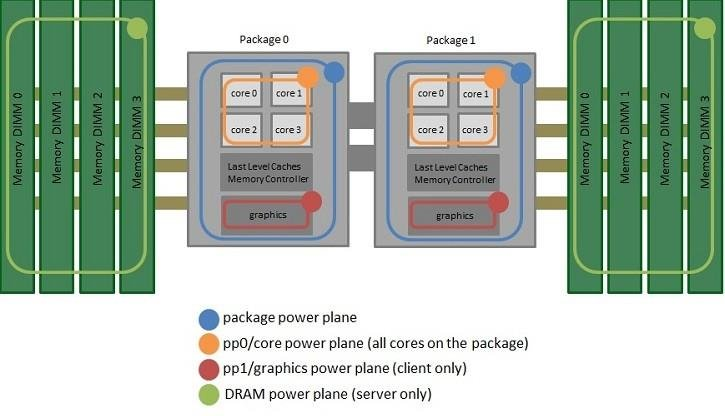
\includegraphics[width=0.8\textwidth]{figures/RAPL-Power-Domains-1.png.jpeg}
    \caption{Esempio di domini di potenza definiti dal modello RAPL. Il dominio
    \textit{Package} rappresenta il consumo energetico complessivo della CPU,
    mentre domini più specifici, come \textit{PP0} e \textit{DRAM}, forniscono
    stime riferite rispettivamente ai core di calcolo e alla memoria principale.}
    \label{fig:rapl-domains}
\end{figure}

Il funzionamento di RAPL si basa su modelli energetici interni al processore,
calibrati dal produttore, che stimano l’energia consumata a partire da eventi
hardware e contatori interni.
Sebbene tali misure non rappresentino una misurazione fisica diretta dell’energia,
diversi studi hanno dimostrato come esse offrano un buon compromesso tra accuratezza
e semplicità di utilizzo, risultando particolarmente adatte al monitoraggio
energetico a runtime\cite{rapl-evaluation}.
Le informazioni rese disponibili da RAPL possono essere lette tramite interfacce
standard del sistema operativo, consentendo la loro integrazione in strumenti di
monitoraggio software.

Nonostante questi vantaggi, i sensori hardware integrati presentano limiti
strutturali quando applicati a contesti software moderni.
La granularità delle misure è tipicamente limitata al livello di macchina o di
componente hardware e non consente di attribuire in modo diretto il consumo
energetico alle singole applicazioni, ai container o alle singole invocazioni.
In ambienti multi-tenant e containerizzati, come quelli tipici del Serverless
Computing, il consumo energetico osservato è quindi il risultato dell’esecuzione
concorrente di più entità software, rendendo complessa l’analisi del comportamento
energetico delle singole funzioni.

Inoltre, le misure fornite da RAPL sono di natura cumulativa e non distinguono in
modo esplicito tra le diverse fasi di esecuzione, quali inizializzazione,
esecuzione vera e propria e periodi di inattività.
Questo aspetto risulta particolarmente critico nel Serverless Computing, dove
fenomeni come il cold start e il riutilizzo dei container hanno un impatto
significativo sul consumo energetico complessivo.
Di conseguenza, pur costituendo una base affidabile per la stima dell’energia a
livello di sistema, i sensori hardware integrati non risultano sufficienti per
supportare analisi a grana fine e decisioni di gestione energetica a livello
software.


Alla luce di queste considerazioni, sebbene i misuratori hardware costituiscano una base affidabile per la misurazione dell’energia, essi risultano insufficienti per
supportare il monitoraggio continuo e a grana fine richiesto da ambienti dinamici e
distribuiti.
In tali contesti emerge la necessità di soluzioni in grado di offrire una maggiore
flessibilità e di integrarsi in modo più stretto con i meccanismi di esecuzione del
software.


\subsection{Misuratori software e modelli di stima}

Le limitazioni intrinseche dei misuratori hardware, quali la scarsa granularità
temporale, i costi elevati di implementazione su larga scala e l’impossibilità di
attribuire direttamente il consumo energetico a singole entità logiche in sistemi
multi-tenant, hanno favorito l’emergere dei misuratori software.
Questi strumenti non si basano su sensori fisici dedicati per ogni applicazione,
ma utilizzano modelli di stima che correlano l’attività del software con il consumo
energetico complessivo del sistema.
Il principio fondamentale consiste nell’impiegare metriche di utilizzo delle
risorse hardware — come cicli di clock della CPU, istruzioni eseguite, accessi alla
cache e operazioni di input/output — come base per stimare l’energia
assorbita dalle singole entità di esecuzione.
Questo approccio consente di ottenere una visibilità energetica più granulare
rispetto alle sole misure hardware, risultando particolarmente adatto a contesti
moderni quali il cloud computing, le architetture a microservizi e i sistemi
containerizzati.

Uno dei framework più rappresentativi in questo ambito è PowerAPI, una libreria modulare progettata per il monitoraggio del consumo energetico a livello di processo attraverso componenti indipendenti e meccanismi di raccolta dati asincroni e scalabili
\cite{fieni:hal-02470128}. L’architettura di PowerAPI è progettata per separare nettamente la fase di raccolta
delle metriche da quella di stima energetica, favorendo l’estendibilità e la
portabilità del sistema. Il pilastro tecnologico di PowerAPI è rappresentato dall’\textbf{HWPC Sensor}
(\textit{Hardware Performance Counter Sensor}), un componente specializzato nel
campionamento ad alta frequenza dei contatori di prestazione hardware
\cite{powerapi-hwpc}.
Il sensore si interfaccia direttamente con il sottosistema \texttt{perf\_event} del
kernel Linux, permettendo di raccogliere metriche dettagliate sull’attività della
CPU associate a specifici \textit{Control Groups} (cgroups)
\footnote{Il sottosistema \texttt{perf\_event} del kernel Linux fornisce
un’interfaccia unificata per il monitoraggio di eventi hardware e software a basso
livello, come cicli di clock della CPU, istruzioni eseguite e cache miss.
Attraverso la chiamata di sistema \texttt{perf\_event\_open()}, consente di associare
le misurazioni a processi, thread o \textit{cgroups}, esponendo i dati tramite
\textit{file descriptor} e buffer ad anello con overhead contenuto.
\texttt{perf\_event} costituisce inoltre la base del tool \texttt{perf}, ampiamente
utilizzato per la profilazione delle prestazioni nei sistemi Linux.} In parallelo, l’HWPC Sensor interroga i \textit{Model Specific Registers} (MSR)
tramite l’interfaccia \textit{Running Average Power Limit} (RAPL), ottenendo misure
cumulative del consumo energetico dei principali domini della CPU
\cite{rapl-evaluation}.

La Figura~\ref{fig:powerapi-architecture} mostra una rappresentazione concettuale
dell’architettura di PowerAPI.
Le metriche di utilizzo delle risorse e le informazioni energetiche fornite dai
sensori hardware vengono elaborate dal modello di stima \textbf{SmartWatts}, adottato
da PowerAPI per attribuire il consumo energetico ai singoli processi.

\begin{figure}[t]
    \centering
    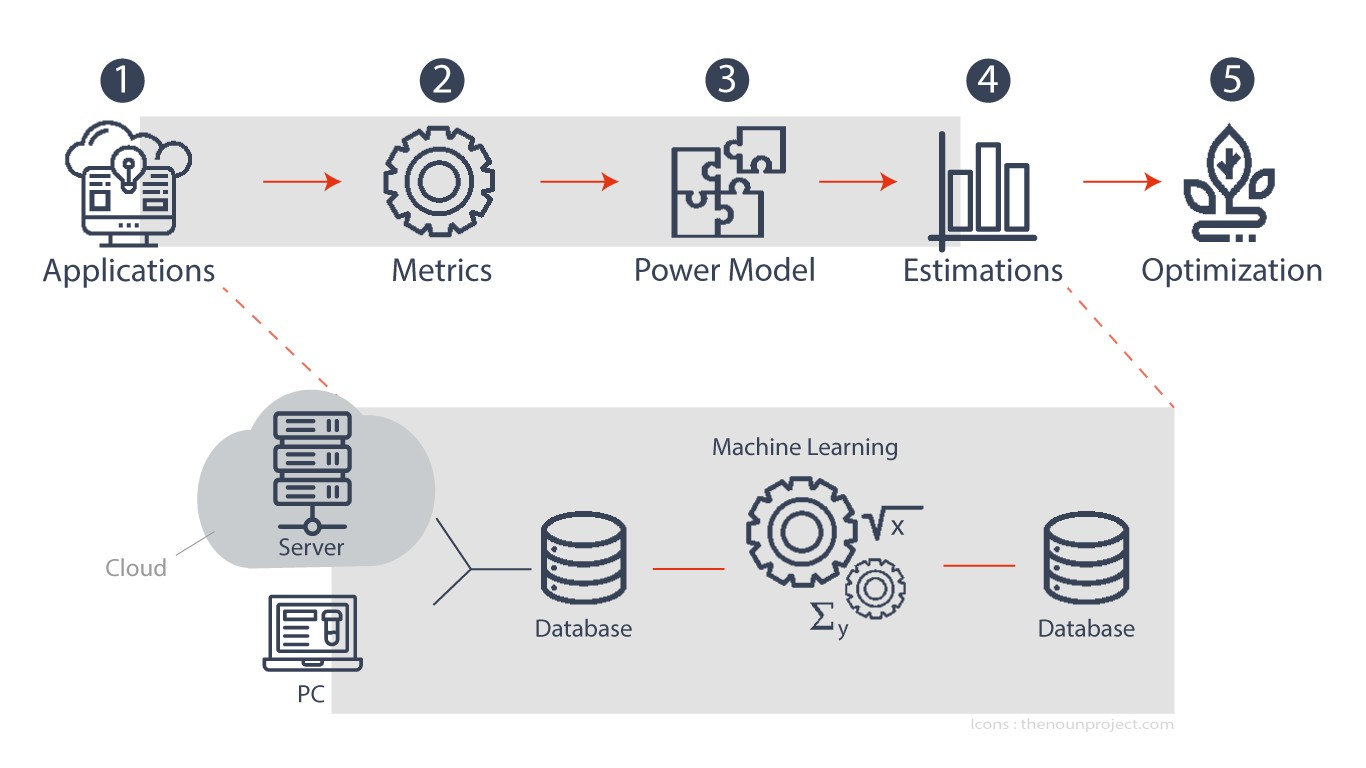
\includegraphics[width=0.9\textwidth]{figures/PowerApi.jpg}
    \caption{Architettura concettuale di PowerAPI. I contatori di prestazione hardware
    e le misure energetiche aggregate (RAPL) vengono combinati dal modello SmartWatts
    per stimare il consumo energetico dei singoli processi.}
    \label{fig:powerapi-architecture}
\end{figure}

SmartWatts utilizza tecniche di regressione lineare per scomporre il consumo
energetico globale in una componente statica e una dinamica, consentendo
un’attribuzione più accurata rispetto a modelli puramente statici
\cite{powerapi-smartwatts}.
Tale approccio richiede una fase di auto-calibrazione \textit{online} e l’accesso
diretto all’hardware sottostante.

Tali requisiti rendono PowerAPI particolarmente adatto a scenari \textit{bare-metal},
ma ne limitano l’applicabilità in ambienti virtualizzati e cloud pubblici, dove
l’accesso ai registri hardware della CPU e ai performance counter è spesso inibito
dagli hypervisor per motivi di sicurezza e isolamento.
In questi contesti emerge la necessità di strumenti di monitoraggio energetico
progettati nativamente per ambienti orchestrati.

Un approccio rappresentativo in questa direzione è \textbf{Kepler}
(\textit{Kubernetes-based Efficient Power Level Exporter}), un progetto
\textit{cloud-native} orientato al monitoraggio energetico di container e Pod in
cluster Kubernetes \cite{kepler-medium,kepler-redhat2}.
A differenza di PowerAPI, Kepler non richiede accesso diretto ai registri hardware
della CPU, ma sfrutta la tecnologia \textit{eBPF} (\textit{Extended Berkeley Packet
Filter}) per raccogliere metriche a livello kernel in modo non intrusivo e con
overhead computazionale ridotto.

La Figura~\ref{fig:kepler-architecture} mostra l’architettura complessiva di Kepler.
Il sistema utilizza un \textit{eBPF Program Generator} per generare dinamicamente
programmi eBPF che vengono agganciati ai \textit{tracepoint} del kernel e ai
performance counter della CPU.
Questi programmi intercettano eventi di schedulazione e statistiche di esecuzione,
consentendo di associare l’attività computazionale ai singoli container in modo
fine-grained.

Le informazioni raccolte tramite eBPF vengono arricchite dal \textit{Pod Lister},
che interroga le API di Kubernetes per mappare gli identificativi dei container ai
rispettivi Pod e raccoglie statistiche aggiuntive dai \textit{control groups}.
Parallelamente, il componente \textit{Energy Stats Reader} acquisisce informazioni
energetiche aggregate dal nodo, utilizzando diverse fonti a seconda della
disponibilità dell’hardware sottostante, tra cui RAPL, sensori hardware esterni,
interfacce GPU (NVML) e modelli basati su benchmark standardizzati.

Quando le misure hardware dirette non risultano accessibili, scenario tipico delle
macchine virtuali nei cloud pubblici, Kepler ricorre a modelli di stima basati su
\textit{Machine Learning}, denominati \textit{Estimators}.
Tali modelli, addestrati offline su differenti architetture hardware e carichi di
lavoro, ricevono in input le metriche raccolte a livello kernel e producono una
stima della potenza assorbita dai container, che viene successivamente integrata nel
tempo per ottenere una stima energetica complessiva.

Le metriche prodotte da Kepler vengono infine esposte tramite un \textit{Prometheus
Exporter}, rendendo il consumo energetico direttamente interrogabile attraverso i
meccanismi di \textit{scraping} standard e facilmente integrabile con strumenti di
visualizzazione.
Questa integrazione nativa con l’ecosistema di osservabilità cloud consente di
affiancare le metriche energetiche a quelle di performance, abilitando analisi
congiunte e politiche di gestione consapevoli dal punto di vista energetico.
\begin{figure}[t]
    \centering
    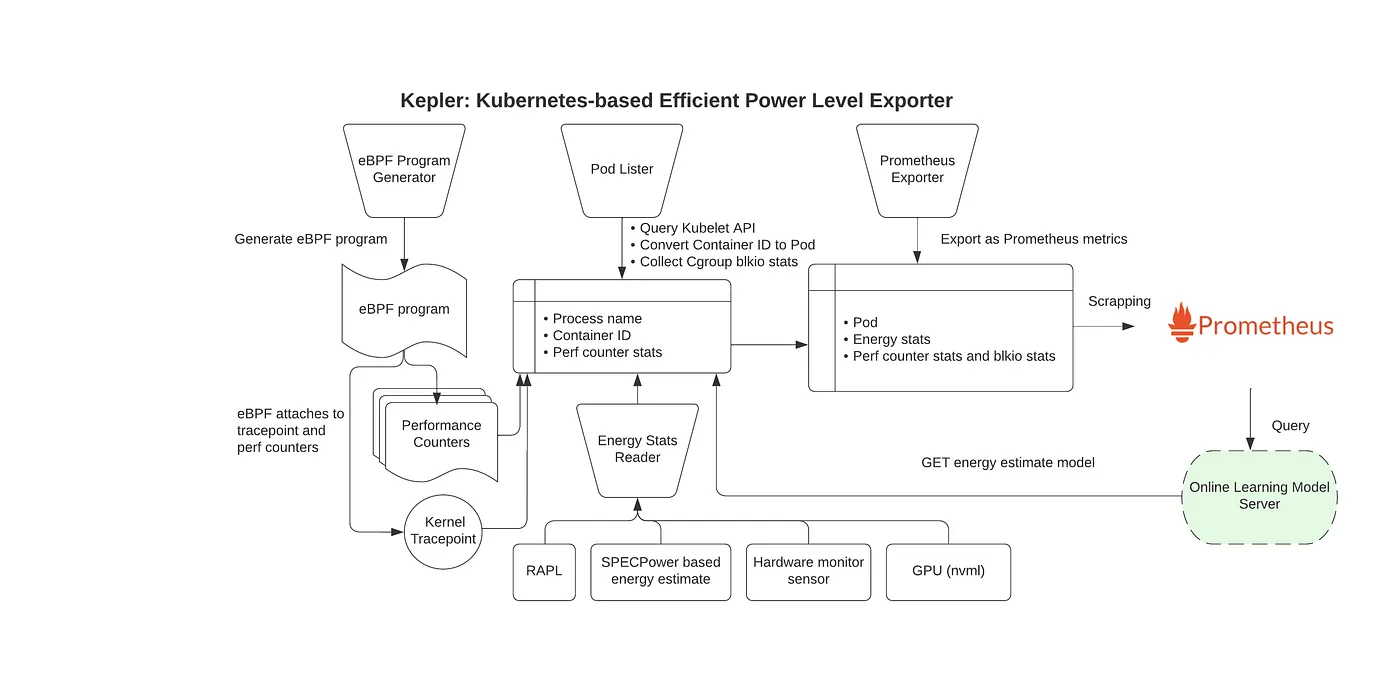
\includegraphics[width=0.75\textwidth]{figures/Kepler.png}
    \caption{Architettura di Kepler.}
    \label{fig:kepler-architecture}
\end{figure}


\section{Elaborazione serverless sostenibile}

Nel paradigma serverless, e in particolare nelle piattaforme 
Function-as-a-Service (FaaS), il consumo energetico è strettamente 
determinato dalla natura del modello di esecuzione: le funzioni sono 
entità effimere, stateless e isolate in ambienti containerizzati, 
invocate su richiesta con cicli di vita che si misurano spesso in 
millisecondi. Tale granularità, combinata con l'elevata variabilità del 
carico di lavoro, rende la gestione dell'energia una dimensione 
strutturalmente più complessa rispetto ai contesti HPC o ai data center 
tradizionali, nei quali le tecniche consolidate operano tipicamente a 
livello di nodo fisico e su scale temporali più ampie.

Allo stato dell'arte, l'efficienza energetica in ambienti serverless è 
affrontata prevalentemente attraverso interventi a livello di 
piattaforma, generalmente trasparenti per l'utente. Le soluzioni più 
diffuse agiscono su tre leve principali: la pianificazione 
energeticamente consapevole delle funzioni (\emph{energy-aware 
scheduling}), la limitazione dinamica della potenza erogata alle risorse 
(\emph{power capping}) e la riduzione dell'impatto energetico associato 
ai tempi di inizializzazione degli ambienti di esecuzione (\emph{cold 
start overhead}).

In questi approcci, il consumo energetico viene trattato come una 
metrica aggiuntiva nel processo decisionale, tipicamente combinata con 
indicatori di prestazione o di qualità del servizio. L'obiettivo è la 
riduzione del consumo medio o complessivo del sistema, senza che vengano 
introdotti vincoli energetici espliciti o meccanismi di garanzia formale 
sul rispetto di un determinato budget. Questa impostazione, sebbene 
efficace in scenari con risorse abbondanti, mostra limiti evidenti in 
contesti caratterizzati da risorse limitate o da stringenti requisiti 
operativi — tra cui ambienti edge — nei quali il consumo energetico non 
può essere trattato come una variabile da ottimizzare in senso 
best-effort, ma deve costituire un vincolo esplicito nel processo di 
pianificazione.

Una direzione complementare, ancora poco esplorata nel contesto 
serverless, consiste nell'agire sulla funzione stessa piuttosto che 
sull'infrastruttura: attraverso il paradigma dell'\emph{Approximate 
Computing}, è possibile generare varianti della medesima funzione che 
riducono il consumo energetico accettando, in modo controllato, una 
diminuzione dell'accuratezza del risultato. Tale approccio sposta il 
problema dalla gestione delle risorse alla progettazione della logica 
applicativa, aprendo la strada a modelli di controllo runtime in grado 
di selezionare dinamicamente il livello di approssimazione più adeguato 
in funzione del budget energetico disponibile.

Nei paragrafi successivi vengono analizzati i principali contributi 
proposti in letteratura, seguendo una progressione che va dagli 
interventi infrastrutturali — scheduling energy-aware e power capping — 
verso meccanismi di controllo applicativo basati su vincoli energetici 
espliciti, delineando il contesto nel quale si inserisce il contributo 
della presente tesi.

\subsection{Scheduling energeticamente consapevole nelle piattaforme FaaS}
\label{subsec:energy_aware_scheduling}

Nel paradigma Function-as-a-Service (FaaS), lo scheduling non costituisce
soltanto un meccanismo di allocazione delle risorse, ma rappresenta uno
strumento strategico per il controllo del consumo energetico
dell'infrastruttura. A differenza delle politiche di pianificazione
tradizionali, orientate prevalentemente all'ottimizzazione delle
prestazioni o al bilanciamento del carico, lo scheduling energeticamente
consapevole integra il consumo energetico tra i criteri che guidano le
decisioni di \emph{placement} e la selezione delle risorse di esecuzione.

Nel contesto serverless, tale problematica presenta caratteristiche
peculiari legate al modello di esecuzione. La breve durata delle
funzioni, la loro natura stateless e l'isolamento in ambienti
containerizzati determinano un'elevata frequenza delle decisioni di
scheduling e una forte sensibilità alle condizioni operative del
momento. In particolare, l'inizializzazione di nuovi ambienti di
esecuzione (\emph{cold start}) può generare picchi di consumo energetico
istantaneo che influenzano in modo non trascurabile l'efficienza
complessiva del sistema; per questa ragione, la gestione del riutilizzo
degli ambienti già attivi (\emph{warm scheduling}) rappresenta una
dimensione rilevante tanto per la latenza percepita quanto per il
profilo energetico medio delle invocazioni.

Un ulteriore elemento di complessità è dato dalla natura distribuita
delle piattaforme FaaS, specialmente in architetture cloud-edge. In
questi scenari, i nodi disponibili per l'esecuzione possono differire
significativamente per capacità computazionale, profilo di consumo,
disponibilità energetica e connettività di rete. Le decisioni di
\emph{placement} devono quindi tenere conto non soltanto delle
prestazioni attese sul singolo nodo, ma anche delle condizioni
energetiche correnti dell'infrastruttura e, in alcuni casi, del costo
associato alla movimentazione dei dati tra siti eterogenei. Questa
molteplicità di fattori rende la progettazione di scheduler
energeticamente consapevoli per piattaforme FaaS un problema
intrinsecamente multi-dimensionale, nel quale le scelte progettuali
riflettono assunzioni diverse sull'architettura, sugli obiettivi di
ottimizzazione e sulle grandezze osservabili a runtime.

L'analisi della letteratura mostra come i contributi proposti in questo
ambito affrontino il problema operando su una leva decisionale comune
--- la scelta del nodo su cui eseguire la funzione --- ma declinandola
in funzione di scenari operativi distinti e con formulazioni
progressivamente più articolate. Nei paragrafi seguenti vengono
analizzati tre approcci rappresentativi, ciascuno dei quali evidenzia
una dimensione specifica della consapevolezza energetica nello scheduling
FaaS.

% ── Faashouse ──────────────────────────────────────────────────────────

In ambienti Edge Computing distribuiti, i nodi possono essere alimentati
da fonti rinnovabili intermittenti --- pannelli solari, micro-turbine
eoliche o batterie con autonomia limitata --- e presentare livelli di
carica variabili nel tempo. In tali contesti, l'obiettivo primario dello
scheduler non è la minimizzazione del consumo medio, bensì il
mantenimento dell'operatività dell'intero sistema, evitando che nodi
con disponibilità energetica residua insufficiente diventino
temporaneamente irraggiungibili o, nel caso peggiore, si spengano
durante l'esecuzione di una funzione.

Il sistema Faashouse~\cite{faashouse}, progettato per ambienti
serverless all'estremo edge, affronta questo problema adottando lo stato
di carica dei nodi (\emph{State of Charge}, SoC) come parametro
decisionale principale per le scelte di \emph{placement}. Come
illustrato in Figura~\ref{fig:faashouse_architecture}, l'architettura
si articola su più livelli --- dispositivi edge a bassa potenza,
piattaforma di containerizzazione e orchestrazione, e livello serverless
per la gestione delle funzioni --- con un \emph{Resource Scheduler}
integrato nel controller che implementa un ciclo di controllo
riconducibile al modello MAPE (\emph{Monitoring, Analyzing, Planning,
Execution}).

\begin{figure}[ht]
    \centering
    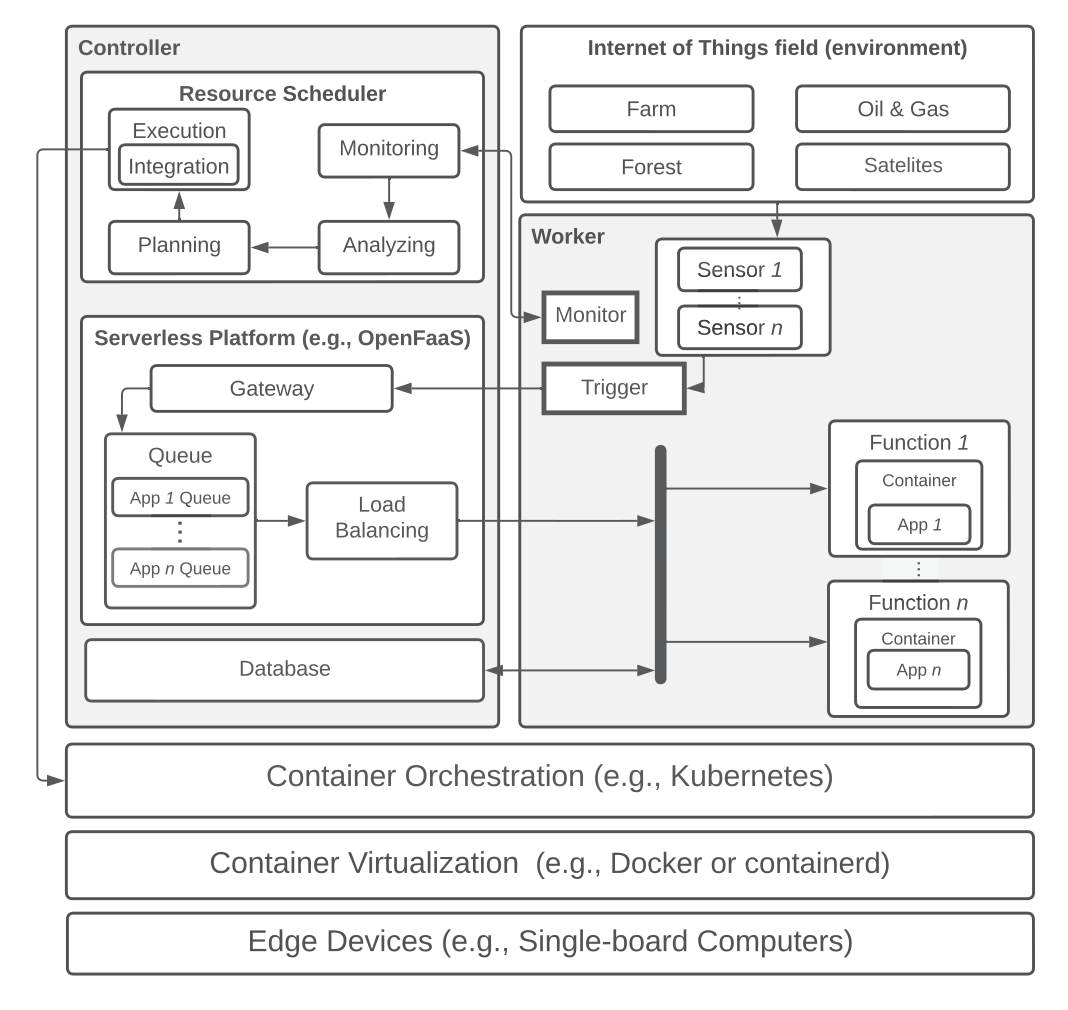
\includegraphics[width=0.9\textwidth]{figures/FaasHouse.png}
    \caption{Architettura del sistema Faashouse. Il controller integra un
    \emph{Resource Scheduler} che, seguendo un ciclo di monitoraggio,
    analisi e pianificazione, decide il \emph{placement} delle funzioni
    sui nodi worker in base allo stato energetico corrente.}
    \label{fig:faashouse_architecture}
\end{figure}

Lo stato energetico di ciascun nodo è una grandezza variabile nel tempo,
determinata congiuntamente dall'energia dissipata durante l'esecuzione
delle funzioni e dall'eventuale energia generata localmente dalle fonti
rinnovabili disponibili. Le decisioni di assegnazione incidono
direttamente sull'evoluzione di tale stato: concentrare le invocazioni
su nodi con SoC ridotto può comprometterne la disponibilità futura,
mentre una redistribuzione bilanciata consente di preservare
l'operatività complessiva dell'infrastruttura. Quando il livello di
carica di un nodo si avvicina a una soglia critica predefinita, le nuove
richieste vengono reindirizzate verso nodi con maggiore disponibilità
energetica mediante meccanismi di \emph{offloading}, realizzando un
bilanciamento energetico dinamico che si adatta alle condizioni
operative correnti.

Questo approccio risulta particolarmente efficace in scenari in cui la
principale fonte di variabilità è la disponibilità energetica
dell'infrastruttura piuttosto che il costo computazionale delle singole
funzioni. Faashouse opera infatti a granularità di nodo e non di
funzione: le invocazioni sono trattate come unità indivisibili, senza
distinzione tra funzioni con profili energetici differenti. Il consumo
energetico per invocazione non è un parametro su cui lo scheduler possa
agire; la sola leva disponibile è la redistribuzione del carico tra
nodi con diversa disponibilità di energia.

% ── E²FIS ──────────────────────────────────────────────────────────────

Se Faashouse affronta il problema della disponibilità energetica
distribuendo le invocazioni tra nodi con capacità residua sufficiente,
un approccio concettualmente diverso consiste nel ridurre il consumo
complessivo dell'infrastruttura attraverso il \emph{workload
consolidation}. In questo modello, lo scheduler non mira a distribuire
uniformemente il carico tra i nodi disponibili, bensì a concentrarlo su
un sottoinsieme selezionato, consentendo ai nodi rimanenti di essere
portati in stato inattivo e, di conseguenza, di non contribuire al
consumo energetico complessivo. L'intuizione alla base di questa
strategia è che il consumo di un nodo in stato di \emph{idle} --- pur
non eseguendo alcuna funzione --- rappresenta una quota non trascurabile
del budget energetico totale, e la sua eliminazione può produrre
risparmi significativi.

Un esempio rappresentativo di questo paradigma è E$^{2}$FIS
(\emph{Energy-Efficient Function Invocation Scheduling})~\cite{e2fis_smartcomp},
proposto per piattaforme FaaS nell'edge--cloud continuum. Il sistema
assume un insieme di nodi eterogenei, ciascuno caratterizzato da
capacità computazionale, memoria disponibile, throughput effettivo e
profilo di consumo energetico. Le funzioni sono descritte tramite
requisiti di memoria, carico computazionale e \emph{deadline} di
completamento; la stima del tempo di esecuzione tiene conto delle
differenze architetturali tra nodi, consentendo allo scheduler di
verificare la compatibilità di ciascuna assegnazione con i vincoli
temporali imposti.

\begin{figure}[ht]
    \centering
    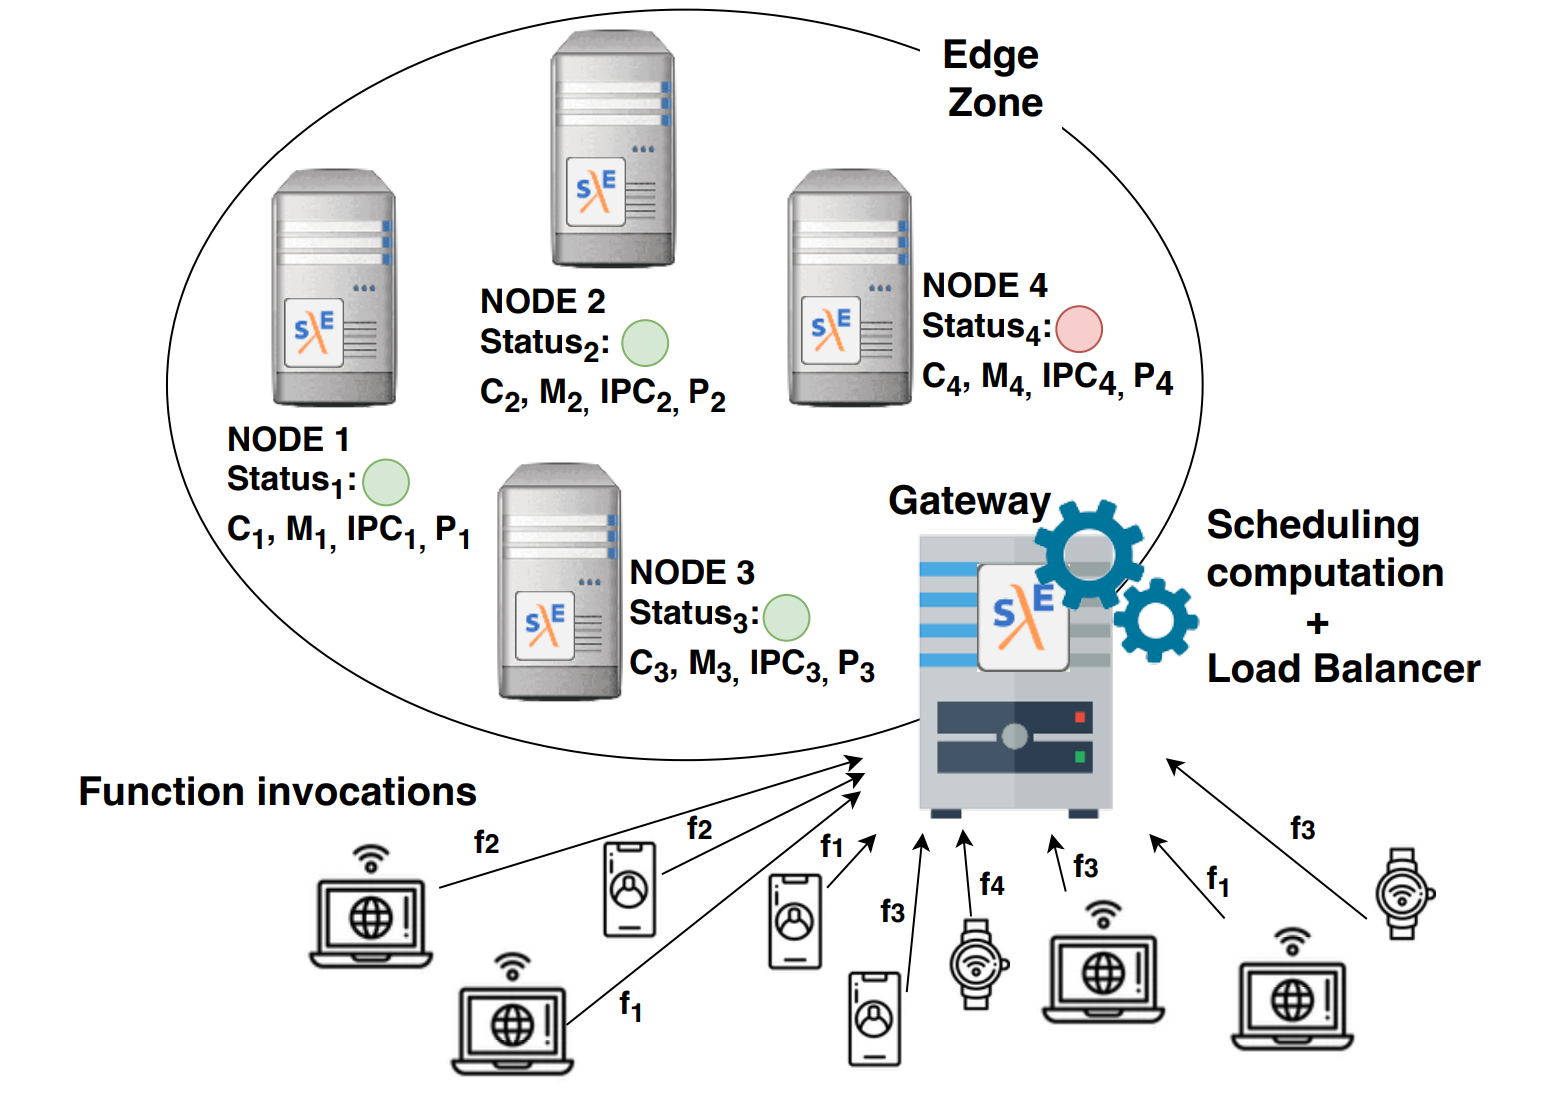
\includegraphics[width=0.85\textwidth]{figures/EnergyEfficientFunctionArchitecture.png}
    \caption{Architettura di E$^{2}$FIS. I nodi edge sono caratterizzati
    da differenti capacità computazionali e profili di consumo. Il modulo
    di \emph{Scheduling computation} determina periodicamente
    l'allocazione delle funzioni e il sottoinsieme di nodi da mantenere
    attivi.}
    \label{fig:e2fis_architecture}
\end{figure}

Come illustrato in Figura~\ref{fig:e2fis_architecture}, l'approccio
adotta una pianificazione periodica basata su epoche temporali discrete.
Prima dell'inizio di ciascuna epoca, il problema di allocazione viene
formulato come un'istanza di Programmazione Lineare Intera Mista (MILP)
e risolto offline. La funzione obiettivo minimizza il consumo energetico
associato ai nodi attivi nell'intervallo considerato, selezionando il
sottoinsieme minimo necessario a soddisfare tutte le richieste entro le
rispettive deadline. Ne deriva una logica di consolidamento: quando il
carico complessivo lo consente, le invocazioni vengono concentrate sui
nodi con il miglior rapporto tra capacità computazionale e consumo
energetico, mentre i restanti possono essere portati in stato inattivo.

Per garantire robustezza operativa in presenza di istanze
computazionalmente onerose o di vincoli particolarmente stringenti, il
sistema prevede un limite temporale per la risoluzione del problema di
ottimizzazione: qualora la soluzione ottima non sia ottenibile entro la
soglia stabilita, viene adottata la migliore soluzione ammissibile
disponibile. In condizioni limite, il framework può inoltre ricorrere a
una politica di fallback ispirata a EDF (\emph{Earliest Deadline
First}), privilegiando il rispetto delle deadline rispetto
all'ottimizzazione energetica. Tale meccanismo evidenzia come, nella
progettazione di scheduler energy-aware, il rispetto dei vincoli
temporali costituisca un obiettivo che, in situazioni di sovraccarico,
assume priorità rispetto all'efficienza energetica, introducendo una
gerarchia esplicita tra gli obiettivi del sistema.

Rispetto a Faashouse, E$^{2}$FIS opera su una leva diversa: anziché
redistribuire il carico in base allo stato energetico corrente dei nodi,
interviene sulla topologia stessa dell'infrastruttura attiva, riducendo
il numero di elementi che contribuiscono al consumo complessivo. Anche
in questo caso, tuttavia, il perimetro decisionale rimane circoscritto
al livello infrastrutturale: lo scheduler seleziona i nodi e assegna le
invocazioni, senza intervenire sulla logica applicativa delle funzioni
eseguite.

% ── GreenFaaS ──────────────────────────────────────────────────────────

I due approcci esaminati finora operano nell'ipotesi che le funzioni
vengano eseguite sullo stesso sito in cui risiedono i dati di input,
o che il costo della loro movimentazione sia trascurabile. In ambienti
FaaS federati o multi-sito, tuttavia, questa assunzione non è sempre
valida. Quando risorse eterogenee e geograficamente distribuite --- tra
cui cluster HPC, workstation e infrastrutture cloud --- partecipano alla
stessa piattaforma di esecuzione, le funzioni possono operare su dataset
residenti in domini amministrativi distinti. In tali scenari, la
decisione di \emph{placement} non dipende soltanto dall'efficienza del
nodo di calcolo, ma anche dal costo energetico necessario a rendere
disponibili i dati di input nel sito selezionato. Ne consegue che
l'allocazione ottimale deve considerare congiuntamente il costo di
\emph{computation} e di \emph{communication}, evitando scelte che
riducono il consumo di esecuzione introducendo al contempo overhead
energetici significativi dovuti alla movimentazione dei dati.

In questo contesto si colloca GreenFaaS~\cite{greenfaas}, un framework
progettato per orchestrare invocazioni FaaS in ambienti distribuiti,
integrando nella decisione di scheduling una stima esplicita del costo
energetico dei trasferimenti. Come mostrato in
Figura~\ref{fig:greenfaas_arch}, l'architettura si articola in tre
componenti principali: un modulo di \emph{Resource Monitoring}, un
\emph{Transfers Manager} e uno \emph{Scheduler}.

\begin{figure}[ht]
    \centering
    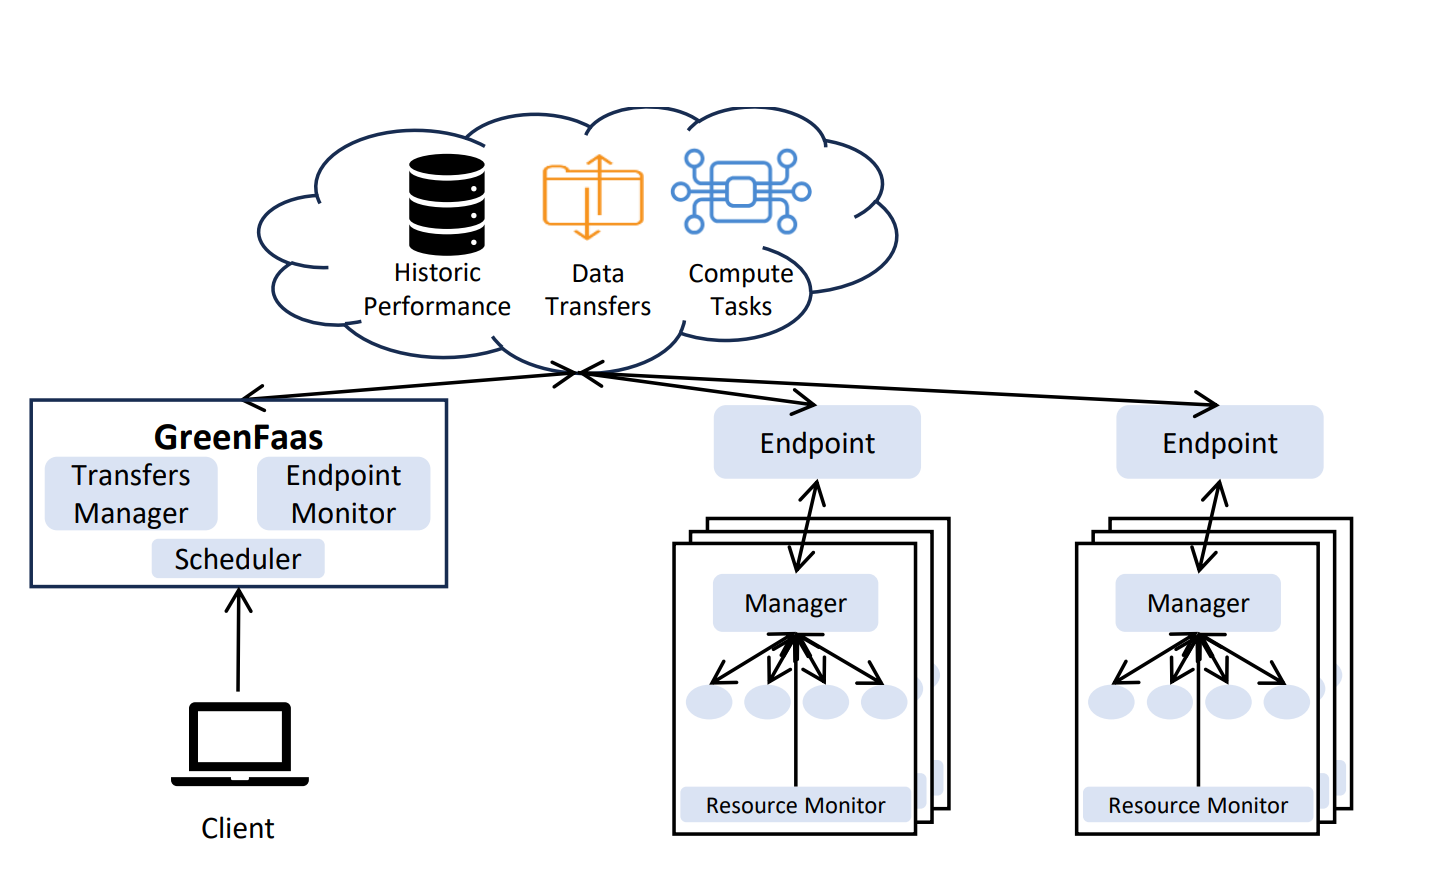
\includegraphics[width=0.9\textwidth]{figures/GreenFaas.png}
    \caption{Architettura di alto livello di GreenFaaS: monitoraggio degli
    endpoint, stima del costo energetico dei trasferimenti e scheduling
    energy-aware per l'allocazione dei task in ambienti federati
    eterogenei.}
    \label{fig:greenfaas_arch}
\end{figure}

Il modulo di monitoraggio raccoglie a runtime metriche energetiche e
prestazionali dei nodi, sfruttando interfacce hardware --- tra cui RAPL
per CPU e NVML per GPU --- per derivare stime di potenza e
caratterizzare il comportamento energetico delle risorse disponibili.
Tali misure consentono di stimare il costo di esecuzione su piattaforme
eterogenee, riducendo la dipendenza da proxy indiretti quali il solo
tempo di esecuzione. Il \emph{Transfers Manager}, a sua volta, modella
il contributo energetico associato alla movimentazione dei dati tra
siti: quando l'input risiede in un dominio diverso da quello candidato
all'esecuzione, il trasferimento introduce un costo legato alla
trasmissione in rete e alle operazioni di I/O agli estremi della
comunicazione. GreenFaaS stima tale costo in funzione della dimensione
dei dati e delle caratteristiche del collegamento, consentendo di
quantificare l'impatto energetico della scelta del sito anche nei casi
in cui il nodo remoto risulti computazionalmente più efficiente.

Sulla base di queste informazioni, lo \emph{Scheduler} effettua una
selezione multi-criterio che integra il consumo energetico previsto per
l'esecuzione sul nodo candidato e il costo energetico dei trasferimenti
eventualmente necessari, affiancando a tali grandezze una stima del
tempo di completamento. Il peso relativo delle componenti è
configurabile, consentendo di modulare il compromesso tra efficienza
energetica e prestazioni in funzione degli obiettivi applicativi. Per
mantenere la reattività in presenza di carichi dinamici e
infrastrutture di grandi dimensioni, il framework adotta strategie
euristiche che evitano un'ottimizzazione globale onerosa.

GreenFaaS amplia dunque la nozione di consapevolezza energetica nello
scheduling FaaS oltre la sola scelta del nodo computazionale,
estendendola al costo di comunicazione tra siti. Questo contributo è
particolarmente rilevante in architetture federali con forte dispersione
geografica, dove i trasferimenti dati possono incidere significativamente
sul bilancio energetico complessivo.

% ── Osservazioni conclusive ────────────────────────────────────────────

Nel complesso, i tre approcci analizzati condividono un elemento
strutturale comune: la decisione di scheduling opera esclusivamente
sulla scelta del nodo di esecuzione, trattando la funzione invocata
come un'entità atomica con un profilo energetico dato. Faashouse
redistribuisce il carico in base alla disponibilità energetica residua
dei nodi; E$^{2}$FIS concentra le invocazioni su un sottoinsieme di
nodi selezionato per minimizzare il consumo complessivo;
GreenFaaS estende la valutazione al costo di comunicazione in ambienti
multi-sito. In nessuno di questi approcci il consumo per singola
invocazione è un parametro su cui lo scheduler possa intervenire: la
funzione viene eseguita nella sua forma originale, indipendentemente
dalle condizioni energetiche del sistema al momento dell'invocazione.

Questa osservazione delimita l'ambito di applicabilità degli approcci
infrastrutturali e motiva l'interesse verso soluzioni che operino a un
livello diverso dello stack di esecuzione, agendo sulla logica
applicativa della funzione piuttosto che sulla selezione del nodo.
Tale direzione è esplorata nelle sezioni successive attraverso il
paradigma dell'Approximate Computing.
\subsection{Power capping come tecnica di controllo energetico}
\label{subsec:power_capping}

Una delle tecniche più consolidate per la gestione del consumo energetico
nei sistemi di calcolo distribuiti è il \emph{power capping}, ovvero
l'imposizione di un limite superiore alla potenza assorbita da uno o
più componenti dell'infrastruttura. A differenza degli approcci orientati
all'ottimizzazione dell'efficienza energetica in senso \emph{best-effort},
il power capping introduce il consumo di potenza come vincolo operativo
esplicito (\emph{hard constraint}), che il sistema non deve violare
durante l'esecuzione dei carichi di lavoro. L'adozione di tali meccanismi
è motivata da vincoli infrastrutturali concreti: i limiti fisici
dell'impianto elettrico, le capacità massime dei sistemi di raffreddamento
o la necessità di operare con budget energetici limitati, come in scenari
Edge o IoT. In letteratura, il problema è classicamente formulato come
un'ottimizzazione vincolata, in cui l'obiettivo consiste nel massimizzare
le prestazioni complessive del sistema nel rispetto di un budget di
potenza prefissato $P_{\max}$.

\subsubsection{Applicabilità degli approcci tradizionali nel contesto serverless}

Approcci consolidati, come quelli analizzati da Ciesielczyk et
al.~\cite{Ciesielczyk2021}, sfruttano leve hardware quali il
\emph{Dynamic Voltage and Frequency Scaling} (DVFS) o interfacce dedicate
come Intel RAPL per modulare dinamicamente la frequenza dei processori e
limitare il consumo di potenza. Tali tecniche si sono dimostrate efficaci
in contesti HPC e in data center tradizionali, operando prevalentemente a
livello di nodo fisico con una granularità temporale relativamente
grossolana.

L'applicazione di questi meccanismi al paradigma serverless introduce
tuttavia criticità specifiche. La natura effimera, \emph{stateless} e
altamente granulare delle funzioni FaaS rende le politiche di capping
statiche spesso poco reattive rispetto alla forte variabilità del carico
di lavoro. Inoltre, il disaccoppiamento tra l'esecuzione delle funzioni e
la gestione diretta delle risorse hardware limita la possibilità di
applicare controlli di potenza con una precisione coerente con la scala
temporale delle invocazioni serverless.

\subsubsection{Impatto sulle prestazioni e approcci adattivi}

L'imposizione di vincoli di potenza in ambienti serverless può comportare
degradazioni delle prestazioni non lineari, riconducibili a due categorie
di effetti ben documentate in letteratura~\cite{Qiu2023PARM}.

La prima riguarda la latenza delle funzioni: esiste una correlazione
diretta tra la riduzione della frequenza della CPU, indotta dal power
capping, e l'aumento della latenza \emph{end-to-end}. Tale effetto è
particolarmente marcato per workload \emph{CPU-bound}, mentre le funzioni
\emph{I/O-bound} risultano meno sensibili, poiché il tempo di esecuzione
è dominato da operazioni di attesa piuttosto che di elaborazione.

La seconda criticità riguarda l'interazione con le politiche di
autoscaling basate su metriche di utilizzo. In presenza di throttling
energetico, il rallentamento dell'esecuzione viene spesso interpretato
come un incremento del carico, inducendo decisioni di scaling subottimali.
Questo comportamento è particolarmente problematico in sistemi adattivi,
dove la non-stazionarietà introdotta dal vincolo di potenza può
compromettere l'efficacia dei meccanismi di apprendimento e di controllo.
La Tabella~\ref{tab:power_capping_effects} sintetizza questi effetti,
evidenziandone l'intensità differenziata in funzione del tipo di workload
e della politica di gestione delle risorse considerata.

\begin{table}[ht]
    \centering
    \caption{Sintesi degli effetti del power capping sulle prestazioni in
    ambienti serverless (rielaborazione basata su~\cite{Qiu2023PARM}).}
    \label{tab:power_capping_effects}
    \renewcommand{\arraystretch}{1.3}
    \begin{tabular}{@{}lp{6cm}l@{}}
        \toprule
        \textbf{Ambito} & \textbf{Effetto osservato} &
        \textbf{Intensità impatto} \\ \midrule
        Latenza CPU-bound & Aumento quasi lineare rispetto alla riduzione
        di frequenza. & Alto \\
        Latenza I/O-bound & Impatto marginale, limitato alle fasi di
        elaborazione. & Basso \\
        Autoscaling & Decisioni subottimali dovute a metriche non
        stazionarie. & Critico \\
        SLO & Incremento delle violazioni degli accordi di servizio.
        & Critico \\ \bottomrule
    \end{tabular}
\end{table}

Per mitigare questi effetti, Qiu et al. propongono PARM
(\emph{Adaptive Resource Allocation for Datacenter Power
Capping})~\cite{Qiu2023PARM}, un framework adattivo che interviene sulla
catena decisionale dell'autoscaling in presenza di vincoli di potenza
attivi. Come illustrato in Figura~\ref{fig:parm_architecture}, PARM
introduce un ciclo di controllo che opera in coordinamento con il
meccanismo di power capping fisico, articolato in due componenti
principali: un \emph{Degradation Predictor}, che stima a runtime
l'impatto del throttling sulle prestazioni applicative, e un
\emph{Resource Re-allocator}, che intercetta e corregge le decisioni
dell'autoscaler prima che vengano applicate al livello di orchestrazione.

\begin{figure}[ht]
    \centering
    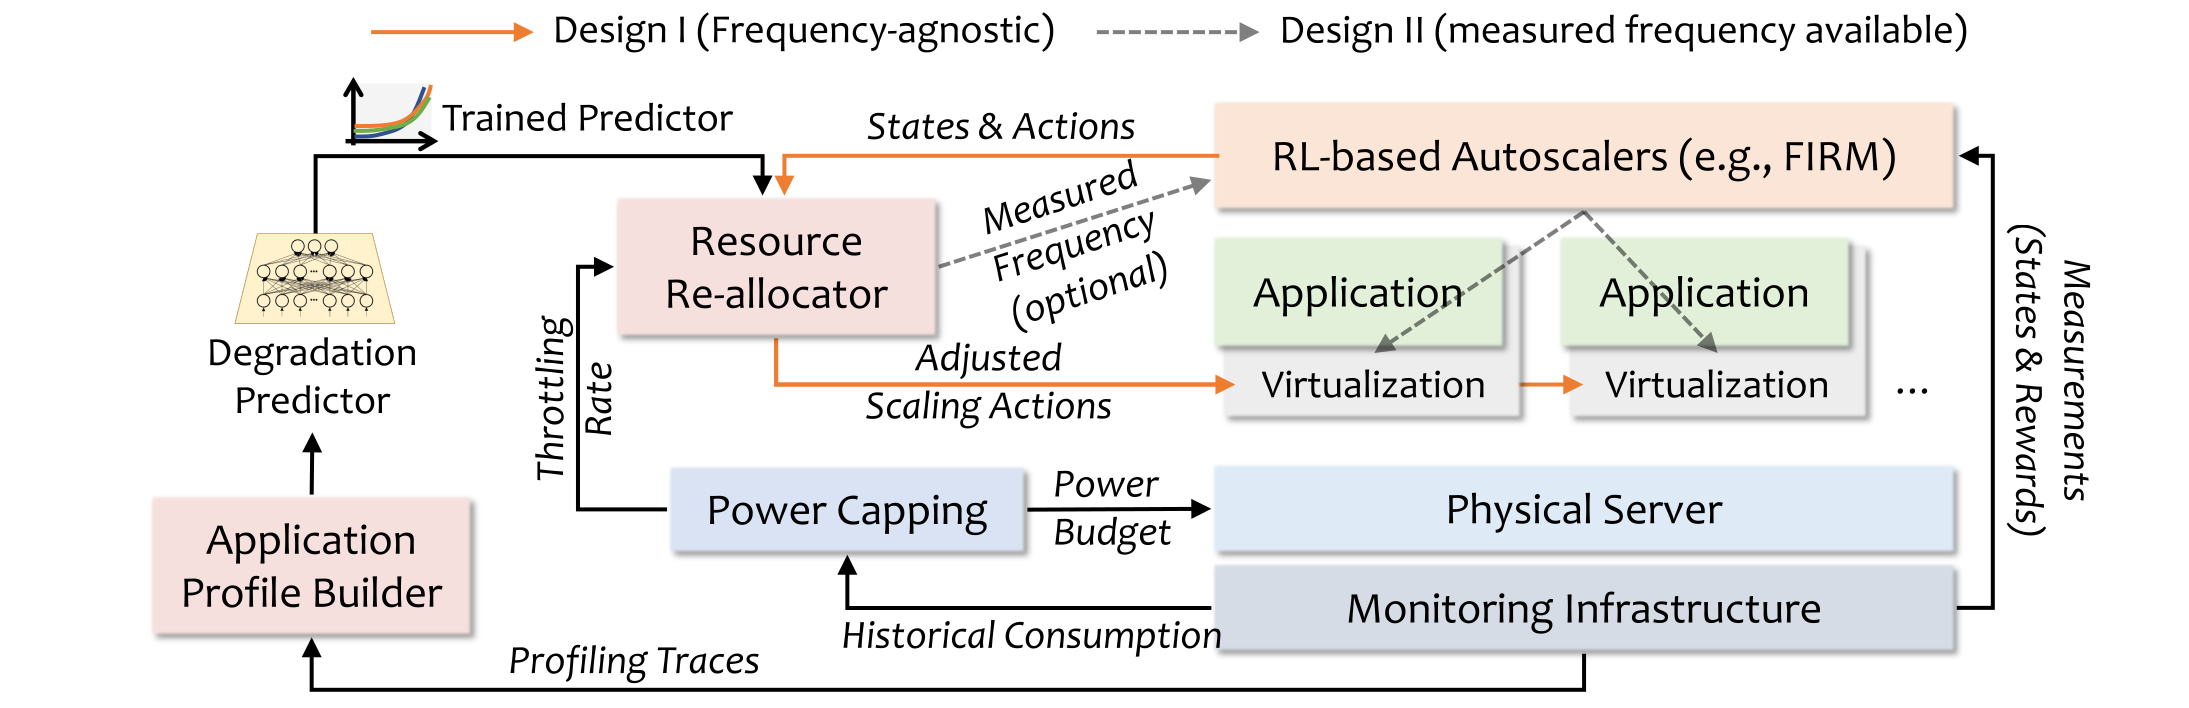
\includegraphics[width=0.9\textwidth]{figures/parm_architecture.png}
    \caption{Schema architetturale del framework PARM. Il
    \emph{Degradation Predictor} stima l'impatto del power capping sulle
    prestazioni, mentre il \emph{Resource Re-allocator} adatta
    dinamicamente le decisioni di scaling in presenza di vincoli di
    potenza.}
    \label{fig:parm_architecture}
\end{figure}

Nel complesso, il power capping rappresenta un meccanismo efficace per
garantire il rispetto di vincoli energetici espliciti, ma la sua
applicazione in ambienti serverless richiede componenti di controllo
adattivo capaci di compensare le distorsioni che il throttling introduce
nei processi decisionali dell'infrastruttura. Gli approcci esaminati
operano prevalentemente a livello hardware e di orchestrazione, agendo
sulla potenza erogata ai nodi o sulle politiche di scaling, senza
intervenire sulla logica di esecuzione delle singole funzioni.
\subsection{Direzioni emergenti per l'elaborazione serverless sostenibile}
\label{subsec:direzioni_sostenibili}

Oltre agli interventi infrastrutturali descritti in precedenza, lo stato
dell'arte evidenzia direzioni complementari volte a rendere l'esecuzione
serverless più sostenibile attraverso meccanismi che agiscono a livello
applicativo piuttosto che infrastrutturale. Anziché intervenire sulla
distribuzione del carico o sulla potenza erogata ai nodi, tali approcci
modificano la relazione tra il comportamento dell'applicazione e il
consumo energetico, introducendo forme di controllo più fine.

Una prima direzione è rappresentata dal paradigma
dell'\emph{Approximate Computing}, che consente di ridurre il consumo
energetico accettando, in modo controllato, una diminuzione
dell'accuratezza del risultato. In questo ambito si colloca
JouleGuard~\cite{jouleguard}, che propone un modello di controllo runtime
capace di rispettare un budget energetico prefissato regolando
dinamicamente il livello di accuratezza dell'applicazione.

\begin{figure}[htbp]
    \centering
    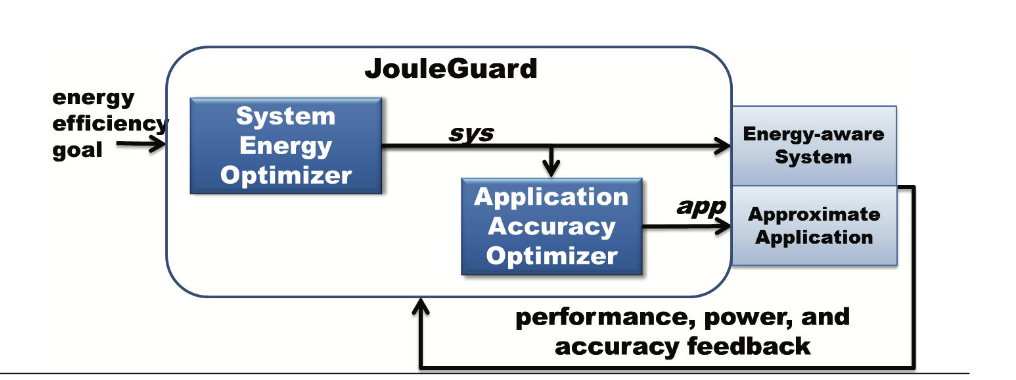
\includegraphics[width=0.8\textwidth]{figures/Jouleguard.png}
    \caption{Schema concettuale di JouleGuard. Il sistema regola
    dinamicamente il livello di accuratezza dell'applicazione in funzione
    di un vincolo energetico esplicito, trattando il budget di potenza
    come parametro attivo nel processo di controllo.}
    \label{fig:jouleguard}
\end{figure}

Come illustrato in Figura~\ref{fig:jouleguard}, il tratto distintivo di
JouleGuard consiste nel trattare l'energia non come una metrica da
minimizzare, ma come un vincolo esplicito che guida il comportamento del
sistema a runtime. La selezione del livello di approssimazione non è
determinata staticamente, ma dipende dalle condizioni operative osservate,
rendendo il sistema adattivo rispetto alla disponibilità energetica
corrente.

Una seconda direzione emerge dal lavoro \emph{Code Once, Run
Green}~\cite{refaas}, che propone di intervenire sull'implementazione
delle funzioni serverless mantenendone invariata la semantica. Gli autori
considerano la medesima funzione logica e ne realizzano una traduzione
automatica verso un linguaggio di programmazione differente,
consentendone l'esecuzione su runtime alternativi con potenziali profili
energetici più favorevoli.

\begin{figure}[htbp]
    \centering
    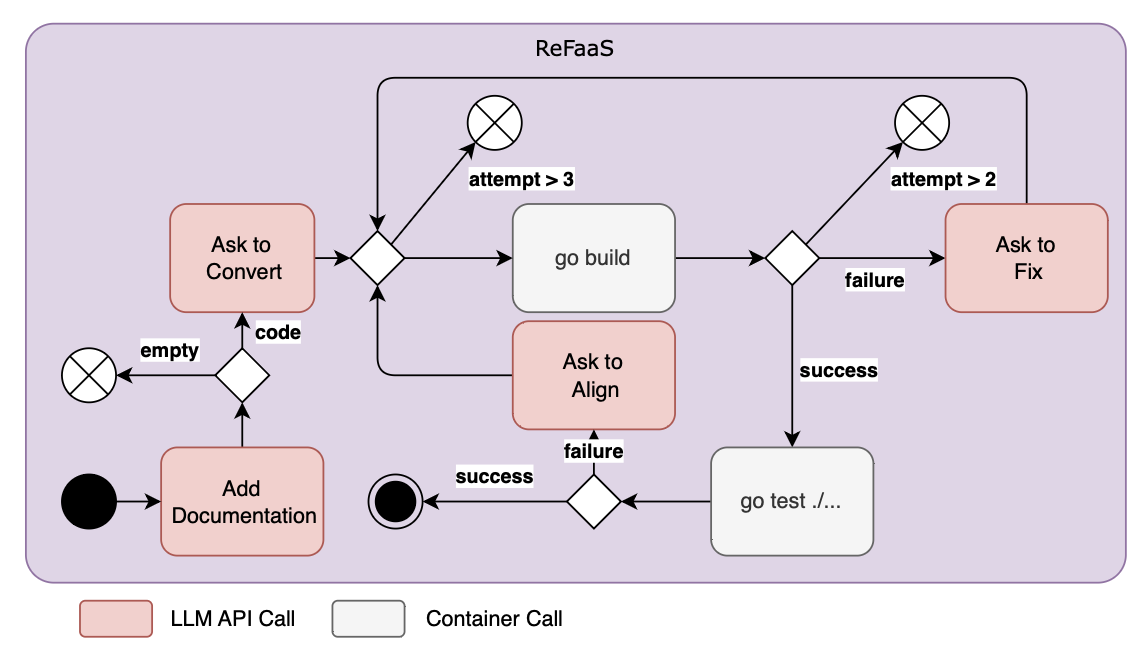
\includegraphics[width=0.85\textwidth]{figures/refaas.png}
    \caption{Pipeline di traduzione automatica proposta in \emph{Code Once,
    Run Green}. La trasformazione avviene in fase di build tramite un
    processo iterativo di conversione e validazione del
    codice.}
    \label{fig:refaas_pipeline}
\end{figure}

Come mostrato in Figura~\ref{fig:refaas_pipeline}, la trasformazione del
codice avviene in fase di build tramite una pipeline di conversione e
validazione iterativa. A differenza dell'approccio di JouleGuard,
l'ottimizzazione energetica è qui perseguita staticamente, agendo sulla
scelta del runtime piuttosto che sul comportamento dell'applicazione
durante l'esecuzione. L'approccio introduce un costo energetico iniziale
associato alla traduzione, potenzialmente ammortizzabile nel tempo
attraverso la riduzione del consumo per invocazione della funzione
tradotta.

Nel loro insieme, i lavori esaminati mostrano come la sostenibilità
dell'elaborazione serverless possa essere perseguita anche al di fuori
degli interventi infrastrutturali, attraverso meccanismi che agiscono
sulla logica applicativa. JouleGuard introduce il concetto di vincolo
energetico esplicito come parametro attivo nel controllo runtime;
\emph{Code Once, Run Green} mostra come la generazione di varianti della
stessa funzione, eseguite su runtime differenti, possa produrre profili
energetici significativamente diversi a parità di semantica.
\section{Il paradigma FaaS in ambienti cloud-edge}
\label{sec:faas_cloud_edge}

Negli ambienti cloud-edge l'elaborazione è distribuita su un insieme
eterogeneo di nodi di calcolo, caratterizzati da differenti capacità
computazionali, disponibilità di memoria, ampiezza di banda e latenza
di rete. Nel paradigma Function-as-a-Service, le applicazioni sono
scomposite in funzioni stateless invocate su richiesta, la cui
esecuzione è demandata alla piattaforma. In un contesto cloud-edge,
ciascuna funzione può essere eseguita localmente su un nodo edge,
oppure instradata verso altri nodi o verso il cloud, in funzione
dello stato delle risorse disponibili al momento dell'invocazione.

Le differenze strutturali tra nodi cloud e nodi edge rendono il
consumo energetico un fattore particolarmente rilevante in questi
scenari. I nodi edge dispongono tipicamente di risorse limitate e
operano in condizioni di maggiore variabilità del carico, spesso
in assenza di infrastrutture di raffreddamento dedicate. Di
conseguenza, le decisioni di allocazione e gestione delle funzioni
non possono basarsi esclusivamente su metriche prestazionali, ma
devono tenere conto dell'impatto energetico delle scelte effettuate,
soprattutto in presenza di vincoli operativi stringenti.

Le tecniche discusse nelle sezioni precedenti — scheduling
energeticamente consapevole, meccanismi applicativi basati su approximate
computing e approcci carbon-aware — sono state sviluppate prevalentemente
in contesti cloud o HPC, con assunzioni sull'infrastruttura che non
sempre si trasferiscono direttamente all'ambiente cloud-edge. In
particolare, la modularità della piattaforma serverless di riferimento
è un requisito determinante: affinché meccanismi di controllo
energetico possano essere integrati senza alterare il modello di
interazione lato utente, l'architettura della piattaforma deve
esporre punti di estensione adeguati a livello di scheduling e
gestione delle funzioni.

In questa prospettiva, la scelta della piattaforma serverless su
cui condurre la sperimentazione non è indifferente. Nella sezione
seguente viene presentata Serverledge, la piattaforma adottata come
riferimento nel presente lavoro, descrivendone le caratteristiche
architetturali rilevanti ai fini della ricerca.

\subsection{La piattaforma Serverledge}
\label{subsec:serverledge}

Serverledge è una piattaforma Function-as-a-Service progettata
per ambienti cloud-edge, caratterizzata da un'architettura
decentralizzata che consente l'esecuzione di funzioni serverless
all'interno di container. La piattaforma separa le componenti di
controllo da quelle di esecuzione, permettendo una gestione
distribuita delle istanze e delle informazioni di stato tra i
nodi che compongono l'infrastruttura.

Ogni nodo Serverledge espone un'interfaccia per la creazione,
l'eliminazione e l'invocazione delle funzioni, supportando sia
la modalità sincrona sia quella asincrona. Le decisioni di
esecuzione sono affidate a uno scheduler, responsabile del
\emph{placement} delle richieste sui nodi disponibili.
L'esecuzione avviene tramite container Docker, mantenuti attivi
per un intervallo di tempo limitato successivamente all'invocazione,
con l'obiettivo di ridurre l'impatto dei \emph{cold start} sulle
invocazioni successive.

La condivisione delle informazioni tra nodi è realizzata tramite
un meccanismo di storage distribuito, che consente di propagare
metadati e informazioni di stato all'interno del cluster. Tali
informazioni sono accessibili dallo scheduler al momento della
decisione di \emph{placement}, permettendo di scegliere tra
l'esecuzione locale sul nodo ricevente e l'offloading verso
altri nodi edge o verso il cloud, in funzione delle condizioni
operative rilevate.

Dal punto di vista architetturale, Serverledge è progettata per
essere estensibile: le logiche di scheduling e di gestione delle
funzioni sono separate dal modello di interazione lato utente,
rendendo possibile l'integrazione di componenti aggiuntivi di
monitoraggio e controllo senza modificare l'interfaccia esposta
agli utenti. Questa proprietà è particolarmente rilevante nel
contesto del presente lavoro, in quanto consente di introdurre
meccanismi di gestione energetica direttamente a livello di
scheduler, sfruttando i punti di estensione nativi della
piattaforma senza alterarne il comportamento di base.
\section{Posizionamento del contributo}
\label{sec:posizionamento}

Le tre famiglie di soluzioni analizzate in questo capitolo ---
scheduling energy-aware, approximate computing e carbon-aware computing
--- operano su dimensioni distinte del problema: la scelta del contesto
di esecuzione, la modulazione della logica applicativa e la sensibilità
al segnale ambientale. Tuttavia, nessuno degli approcci esaminati le
integra in un unico meccanismo decisionale.

In particolare, nessuno degli approcci esaminati affronta il problema
di selezionare, al momento dell'invocazione, la variante di una
funzione che offra il miglior compromesso tra consumo energetico e
accuratezza del risultato in funzione dell'impatto ambientale corrente
dell'esecuzione. Manca un meccanismo che utilizzi la carbon intensity
non come criterio di \emph{placement} geografico o temporale, ma come
segnale per modulare il punto operativo sul trade-off
energia-accuratezza della funzione stessa --- spostando la selezione
verso varianti a minor consumo quando la rete è alimentata da fonti ad
alta intensità di carbonio, e verso varianti a maggiore accuratezza
quando le condizioni della rete lo consentono.

A ciò si aggiunge una seconda lacuna, trasversale agli approcci
esaminati: in ambienti FaaS, il consumo energetico di una funzione non
è una grandezza stabile nel tempo, ma varia in funzione del carico
concorrente sul nodo, dello stato del container e delle caratteristiche
dei dati di input. Fondare le decisioni di selezione su profili
energetici determinati offline significa operare su stime
potenzialmente disallineate rispetto alle condizioni operative correnti,
con conseguenze dirette sull'efficacia del meccanismo decisionale.

Il presente lavoro si propone di colmare questo spazio, integrando le
tre dimensioni identificate in un unico sistema di scheduling che
operi a livello di singola invocazione, selezionando tra varianti della
stessa funzione sulla base di stime energetiche aggiornate
continuamente e di un segnale di carbon intensity contestualizzato
rispetto alla zona geografica di esecuzione.
\chapter{Progettazione e Realizzazione}
\label{cap:ProgettazioneRealizzazione}

\emph{In questo capitolo vengono descritte le scelte progettuali e i meccanismi 
realizzati per estendere Serverledge con capacità di monitoraggio e 
schedulazione energeticamente consapevole. Viene dapprima introdotto il 
modello di funzione logica con varianti energetiche, che costituisce 
l'astrazione fondamentale su cui si basa l'intero sistema. Si descrive 
quindi l'integrazione di Kepler per la misurazione dei consumi a livello 
di container e il worker periodico responsabile dell'aggiornamento adattivo 
dei profili energetici delle varianti. Infine, viene illustrata la logica 
decisionale dello scheduler energy-aware, progettato per selezionare a 
runtime la variante più accurata nel rispetto di un eventuale vincolo 
energetico, subordinatamente al consenso esplicito dell'utente.}
\section{Integrazione di Kepler per il monitoraggio energetico}

Il monitoraggio dei consumi energetici a livello di container costituisce 
il fondamento del sistema realizzato. A tal fine è stato adottato Kepler 
(Kubernetes-based Efficient Power Level Exporter), uno strumento open 
source sviluppato nell'ambito della CNCF (Cloud Native Computing 
Foundation) che stima il consumo energetico di processi, container e 
pod Kubernetes attraverso l'accesso diretto alle interfacce hardware del 
sistema operativo host~\cite{keplerCNCF2023}.

La scelta di Kepler è motivata principalmente dalla sua granularità di 
misurazione, che opera a livello di singolo container Docker: questa 
corrisponde esattamente all'unità di esecuzione delle funzioni serverless 
in Serverledge. Kepler espone inoltre le proprie metriche nel formato 
standard Prometheus, consentendo un'integrazione diretta con l'ecosistema 
di monitoraggio senza richiedere componenti aggiuntivi per la raccolta 
dei dati.

\subsection{Funzionamento di Kepler}

Kepler opera combinando due meccanismi complementari per associare i 
consumi energetici ai singoli container. Il primo è un programma eBPF 
(Extended Berkeley Packet Filter) integrato nel kernel, che traccia 
l'attività dei processi e li associa ai container tramite il file 
\texttt{/proc/PID/cgroup}, consentendo di correlare il Process ID di 
ciascun processo all'identificatore del container che lo ospita. Il 
secondo è l'interfaccia RAPL (Running Average Power Limit), disponibile 
sui processori Intel e AMD moderni, che permette di leggere i contatori 
energetici cumulativi direttamente dai registri hardware della CPU.

Una volta raccolti i dati di utilization dei processi e di consumo 
energetico del sistema, Kepler applica il \emph{Ratio Power Model} per 
attribuire a ciascun container la propria quota di consumo: la potenza 
dinamica viene distribuita tra i container in proporzione alla loro 
utilization rispetto all'utilization totale del sistema. Il risultato 
viene aggregato a livello di container e reso disponibile tramite 
Prometheus nella metrica \texttt{kepler\_container\_cpu\_joules\_total}, 
un contatore cumulativo espresso in Joule che cresce monotonicamente nel 
tempo per ogni container attivo.

\begin{figure}[ht]
    \centering
    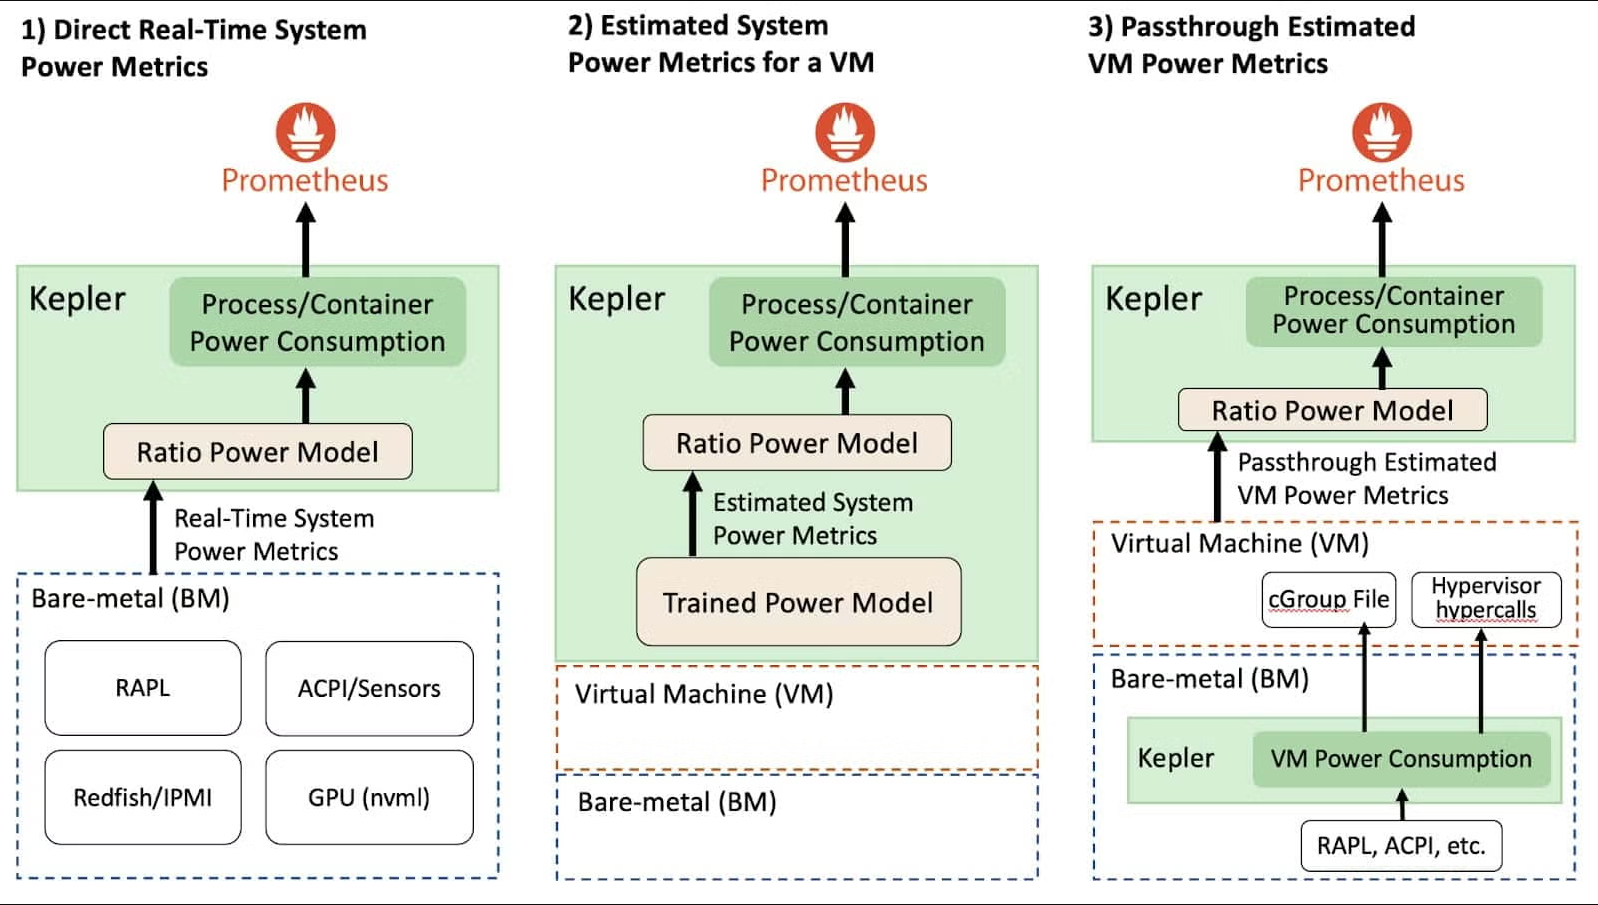
\includegraphics[width=0.85\textwidth]{figures/KeplerArchitecture.jpg}
    \caption{Architettura di Kepler per la raccolta dei consumi energetici 
    in ambienti bare-metal e virtuali. In ambienti bare-metal, Kepler 
    accede direttamente ai contatori hardware tramite RAPL, ottenendo 
    misurazioni real-time senza necessità di modelli predittivi. }
    \label{fig:kepler-arch}
\end{figure}

Come illustrato in Figura~\ref{fig:kepler-arch}, il comportamento di
Kepler varia in base all'ambiente di esecuzione. In ambienti bare-metal,
Kepler accede direttamente ai contatori RAPL, ottenendo misurazioni
energetiche real-time senza ricorrere a modelli predittivi
pre-addestrati. In ambienti virtualizzati, invece, l'assenza di accesso
diretto all'hardware richiede l'uso di modelli di regressione,
introducendo le relative limitazioni di accuratezza.

Per accedere alle interfacce hardware necessarie, Kepler deve essere 
eseguito con privilegi elevati sull'host: richiede accesso a 
\texttt{/sys} e \texttt{/proc} per leggere i contatori RAPL e i cgroup, 
e al socket Docker per identificare i container attivi e associarvi le 
metriche energetiche.

\subsection{Infrastruttura di supporto}

L'avvio dell'infrastruttura di monitoraggio è gestito dallo script 
\texttt{StartMetrics.sh}, che inizializza come container Docker tutti 
i servizi necessari al funzionamento del sistema.  
\begin{figure}[H]
    \centering
    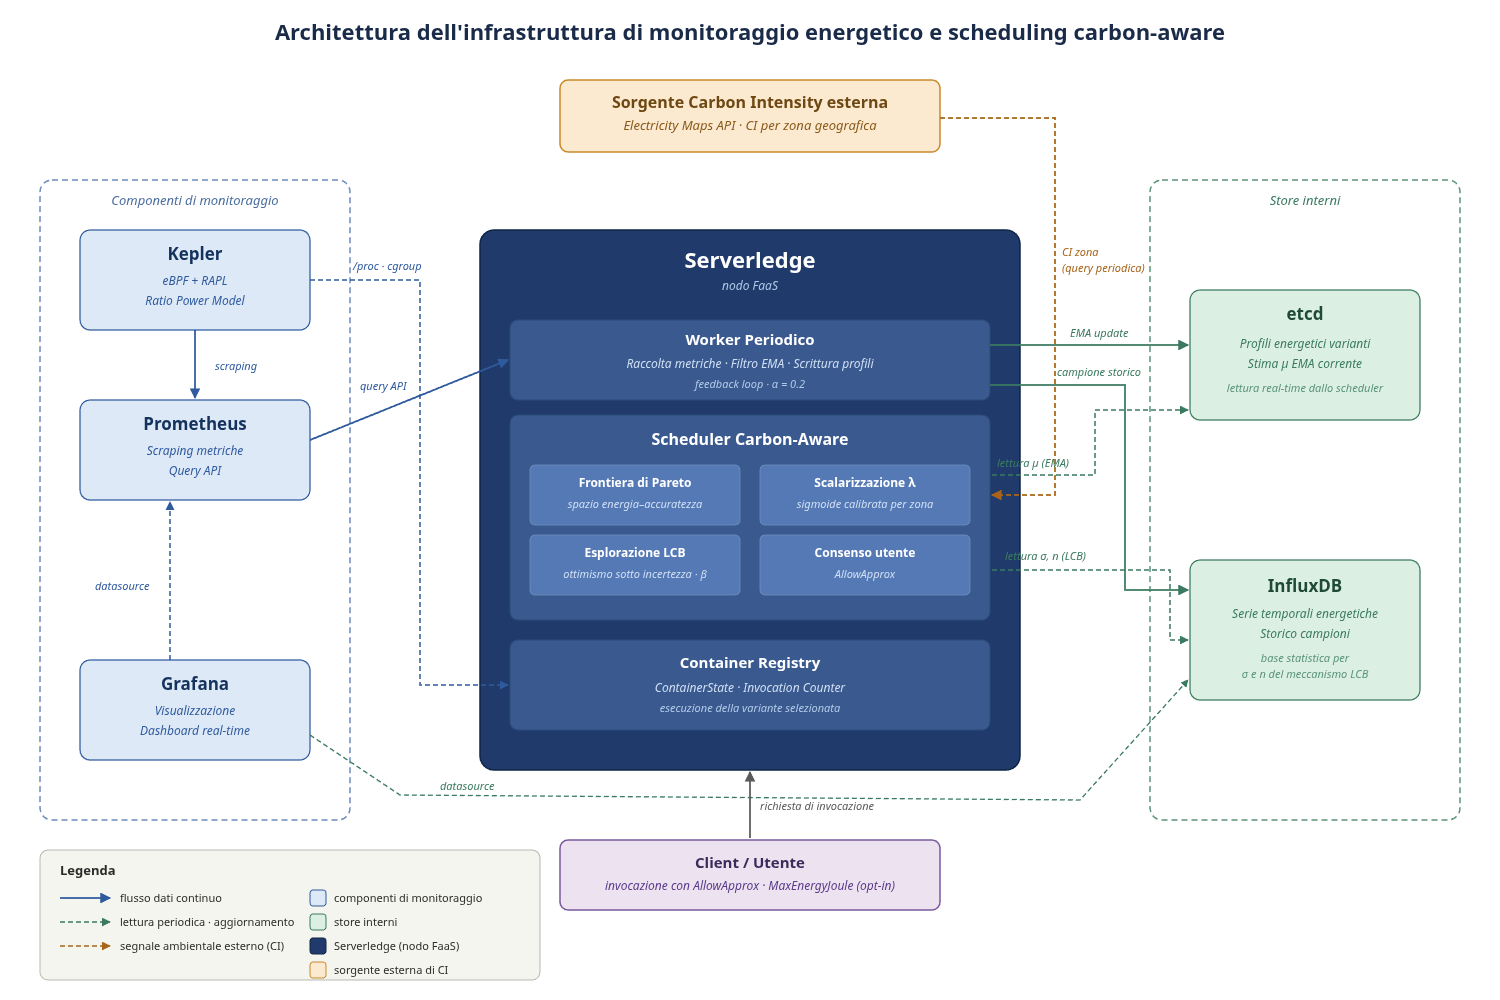
\includegraphics[width=0.85\textwidth]{figures/infrastracture-diagram.png}
    \caption{Architettura dell'infrastruttura di monitoraggio energetico e scheduling
carbon-aware. I componenti di monitoraggio esterni (Kepler, Prometheus, Grafana)
sono separati dagli store interni (etcd, InfluxDB), con Serverledge al centro
che interagisce con entrambi i livelli. Lo scheduler carbon-aware integra la
logica di selezione della variante — basata su frontiera di Pareto, scalarizzazione
tramite $\lambda$, esplorazione LCB e consenso utente — e riceve il segnale di
carbon intensity tramite query periodica a una sorgente esterna.}
    \label{fig:infra-arch}
\end{figure}

I componenti avviati,  come mostrato anche in Figura~\ref{fig:infra-arch}, sono i seguenti:

\begin{itemize}
    \item \textbf{Kepler}: eseguito in modalità privilegiata con accesso
 a \texttt{/sys}, \texttt{/proc} e al socket Docker dell'host, 
    condizioni necessarie per la lettura dei contatori RAPL e 
    l'associazione dei consumi ai container tramite cgroup.
    
    \item \textbf{Prometheus}: configurato per effettuare lo scraping 
    periodico delle metriche esposte da Kepler, rendendole disponibili 
    tramite API di interrogazione.
    
    \item \textbf{InfluxDB}: database a serie temporali utilizzato per 
    l'archiviazione storica dei campioni energetici prodotti dal 
    sistema ad ogni ciclo di raccolta.
    
    \item \textbf{etcd}: store distribuito chiave-valore che funge da 
    registro delle funzioni e delle relative varianti, inclusi i profili 
    energetici aggiornati dinamicamente a runtime.
    
    \item \textbf{Grafana}: strumento di visualizzazione utilizzato per 
    il monitoraggio in tempo reale dei consumi durante gli esperimenti.
\end{itemize}

Una volta avviata, l'infrastruttura opera in modo autonomo: Kepler 
rileva i container Docker presenti sull'host e ne aggiorna le metriche 
energetiche ad ogni ciclo di campionamento; Prometheus le raccoglie e 
le rende interrogabili; il sistema interno di Serverledge, descritto nelle sezioni successive,
le legge periodicamente --- limitatamente ai container attivi da esso gestiti --- per aggiornare i profili energetici 
delle varianti di funzione. Il segnale di carbon intensity, necessario allo scheduler 
per la selezione carbon-aware della variante, non è parte di questa infrastruttura: 
viene acquisito dallo scheduler a runtime tramite query periodica a una 
sorgente esterna, come descritto nella Sezione~\ref{cap:scheduler}.
\section{Il modello di funzione logica con varianti}
\label{sec:variant-model}

Il supporto all'esecuzione energeticamente consapevole richiede che il 
sistema possa rappresentare, per una stessa funzione, implementazioni 
alternative con diversi profili di consumo e accuratezza. A tal fine è 
stato introdotto il concetto di \emph{funzione logica con varianti}: 
un'astrazione che raggruppa sotto un unico identificatore logico più 
implementazioni della stessa funzione, ciascuna caratterizzata da un 
proprio profilo energetico e da un modello di output che ne quantifica 
l'accuratezza.

\subsection{Struttura della funzione e profilo energetico}

In Serverledge, ogni funzione è rappresentata dalla struttura 
\texttt{Function}, estesa in questo lavoro con i campi necessari al 
supporto delle varianti energetiche. I campi rilevanti per il sistema 
proposto sono i seguenti:

\begin{itemize}
    \item \texttt{LogicalName}: identificatore condiviso da tutte le 
    varianti appartenenti alla stessa funzione logica. Costituisce 
    il riferimento con cui il client invoca la funzione, 
    indipendentemente dalla variante che verrà selezionata a runtime.

    \item \texttt{VariantID}: identificatore univoco della specifica 
    variante all'interno del gruppo logico (ad esempio \texttt{base}, 
    \texttt{light}, \texttt{c}).

    \item \texttt{EnergyProfile}: struttura che mantiene la stima 
    energetica della variante, composta da due campi:
    \begin{itemize}
        \item \texttt{ColdStartJoule}: energia stimata per l'avvio a 
        freddo del container, comprensiva dell'inizializzazione del 
        runtime;
        \item \texttt{InvocationJoule}: energia media stimata per una 
        singola invocazione della funzione
    \end{itemize}
    \item \texttt{AllowApprox}: flag booleano che indica se la funzione 
    logica ammette l'utilizzo di varianti approssimate. La sua 
    attivazione è condizione necessaria affinché lo scheduler 
    energy-aware possa considerare varianti con accuratezza ridotta.
\end{itemize}

\input{src/subsubsection/chapter3/section2/01-DeterminazioneProfiliEnergeticiIniziali}
\subsection{Il modello di output e la classificazione dell'accuratezza}
\label{sec:output-model}

Per consentire allo scheduler di confrontare le varianti in termini di 
accuratezza, ciascuna variante è dotata di un \texttt{OutputModel} che 
descrive la qualità del suo output. Il modello supporta due tipologie 
di classificazione, scelte in base alla natura computazionale della 
funzione:

\begin{itemize}
    \item \textbf{Tipo \texttt{error}}: adatto a funzioni il cui output 
    è un valore numerico misurabile. L'accuratezza è espressa tramite 
    il campo \texttt{error\_estimate}, che rappresenta l'errore relativo 
    atteso rispetto alla variante di riferimento. Una variante esatta 
    presenta \texttt{error\_estimate = 0.0}, mentre varianti approssimate 
    presentano valori positivi proporzionali alla deviazione introdotta 
    dalla semplificazione algoritmica adottata.

    \item \textbf{Tipo \texttt{quality}}: adatto a funzioni il cui 
    output non è facilmente quantificabile con un errore numerico, 
    come classificatori o modelli di machine learning. L'accuratezza 
    è espressa tramite un livello discreto: \texttt{high}, 
    \texttt{medium} o \texttt{low}, che riflette la qualità complessiva 
    del risultato prodotto dalla variante.
\end{itemize}

Il ~\autoref{lst:imageclassification-json} mostra un esempio 
applicativo del tipo \texttt{quality} per la funzione 
\texttt{ImageClassification}, in cui la variante base utilizza un 
modello di rete neurale più accurato ma più oneroso, mentre la 
variante \texttt{Light} adotta un modello più compatto a qualità ridotta.

\begin{lstlisting}[
    language=json,
    caption={File di definizione delle varianti per la funzione 
    \texttt{ImageClassification}. Il campo \texttt{quality} esprime 
    l'accuratezza in forma discreta, adatta a output non numericamente 
    quantificabili.},
    label={lst:imageclassification-json}
]
{
  "variants": [
    {
      "id": "base",
      "runtime": "python-ml",
      "entry_point": "ImageClassification.handler",
      "src": "ImageClassification.py",
      "energy": {
        "cold_start_joule": 1.894736842,
        "invocation_joule": 1.455263158
      },
      "output": { "type": "quality", "quality": "high" },
      "is_approximate": false
    },
    {
      "id": "Light",
      "runtime": "python-ml",
      "entry_point": "ImageClassificationLight.handler",
      "src": "ImageClassificationLight.py",
      "energy": {
        "cold_start_joule": 1.071052329,
        "invocation_joule": 0.22894768
      },
      "output": { "type": "quality", "quality": "low" },
      "is_approximate": true
    }
  ]
}
\end{lstlisting}

Lo scheduler converte internamente entrambe le rappresentazioni in un 
punteggio numerico (\emph{ErrorScore}) secondo una scala uniforme: 
per il tipo \texttt{error} viene utilizzato direttamente il valore di 
\texttt{error\_estimate}, mentre per il tipo \texttt{quality} i livelli 
\texttt{high}, \texttt{medium} e \texttt{low} vengono mappati 
rispettivamente a $0.0$, $1.0$ e $2.0$. La selezione privilegia 
sempre la variante con il punteggio più basso compatibile con il 
vincolo energetico, garantendo che la qualità del risultato sia 
massimizzata nei limiti imposti dalla richiesta.

La Tabella~\ref{tab:output-models} riassume il modello di output 
adottato per ciascuna delle funzioni utilizzate negli esperimenti.

\begin{table}[h]
    \centering
    \begin{tabular}{llll}
        \toprule
        \textbf{Funzione} & \textbf{Tipo} & 
        \textbf{Variante base} & \textbf{Variante approssimata} \\
        \midrule
        Fibonacci         & \texttt{error}   & 0.0  & 0.0 \\
        PiLeibniz         & \texttt{error}   & 0.0  & $1.99 \times 10^{-8}$ \\
        Sqrt              & \texttt{error}   & 0.0  & 0.043 \\
        VectorMagnitude   & \texttt{error}   & 0.0  & 0.04 \\
        SentimentAnalysis & \texttt{quality} & high & low \\
        ImageClassification & \texttt{quality} & high & low \\
        \bottomrule
    \end{tabular}
    \caption{Modello di output adottato per ciascuna funzione. Per il 
    tipo \texttt{error} il valore riportato è \texttt{error\_estimate}; 
    per il tipo \texttt{quality} il livello discreto assegnato.}
    \label{tab:output-models}
\end{table}
\subsection{Registrazione e indicizzazione delle varianti in etcd}
\label{sec:variant-registration}

Le varianti di una funzione logica vengono definite tramite un file 
JSON collocato nella directory \texttt{variants/<LogicalName>/} del 
progetto. Al momento della registrazione, il sistema legge questo file 
attraverso il componente \texttt{FileSource}, prepara il codice 
sorgente di ciascuna variante in formato tar e materializza le varianti 
in etcd attraverso la funzione \texttt{CreateInternalVariants}.

\subsubsection{Convenzione di denominazione}

La convenzione di denominazione distingue la variante di riferimento 
dalle varianti alternative. La prima variante definita nel file JSON, tipicamente quella a massima accuratezza, mantiene come nome interno 
esattamente il \texttt{LogicalName}, preservando la compatibilità con 
le invocazioni che non specificano alcuna preferenza energetica. Le 
varianti successive ricevono un nome composto nella forma 
\texttt{<LogicalName>-<VariantID>}. Per la funzione logica 
\texttt{fibonacci} (\autoref{lst:fibonacci-json}) ad esempio, i nomi interni assegnati sono:

\begin{itemize}
    \item \texttt{fibonacci} — variante base in Python
    \item \texttt{fibonacci-optimization-py} — variante ottimizzata 
    in Python
    \item \texttt{fibonacci-c} — variante compilata in C nativo
\end{itemize}

\subsubsection{Struttura delle chiavi in etcd}

Il sistema mantiene in etcd due livelli distinti di chiavi, ciascuno 
con una responsabilità specifica, come illustrato in 
Figura~\ref{fig:etcd-structure}.

Il primo livello, sotto il prefisso \texttt{/function/}, contiene una 
chiave per ogni variante registrata nel sistema, indipendentemente 
dalla funzione logica di appartenenza. Il valore associato è la 
serializzazione JSON completa della struttura \texttt{Function}, che 
include il runtime, il codice sorgente, il profilo energetico corrente 
e il modello di output. È su queste chiavi che il worker periodico 
scrive gli aggiornamenti del campo \texttt{InvocationJoule} ad ogni 
ciclo di raccolta.

Il secondo livello, sotto il prefisso 
\texttt{/index/logical/<LogicalName>/}, costituisce un indice che 
associa ciascun nome logico all'insieme delle sue varianti. La 
motivazione di questo indice è di natura prestazionale: poiché la 
selezione della variante avviene nel critical path della richiesta di 
invocazione, è necessario che lo scheduler possa recuperare 
rapidamente tutte le varianti di una funzione logica senza dover 
scorrere l'intero prefisso \texttt{/function/}, che contiene tutte 
le funzioni registrate nel sistema. Tramite l'indice, il recupero 
avviene con una singola query con prefisso su 
\texttt{/index/logical/<LogicalName>/}, restituendo esclusivamente le 
varianti della funzione richiesta e contenendo così la latenza 
introdotta dalla fase di selezione a runtime.

\begin{figure}[H]
    \centering
    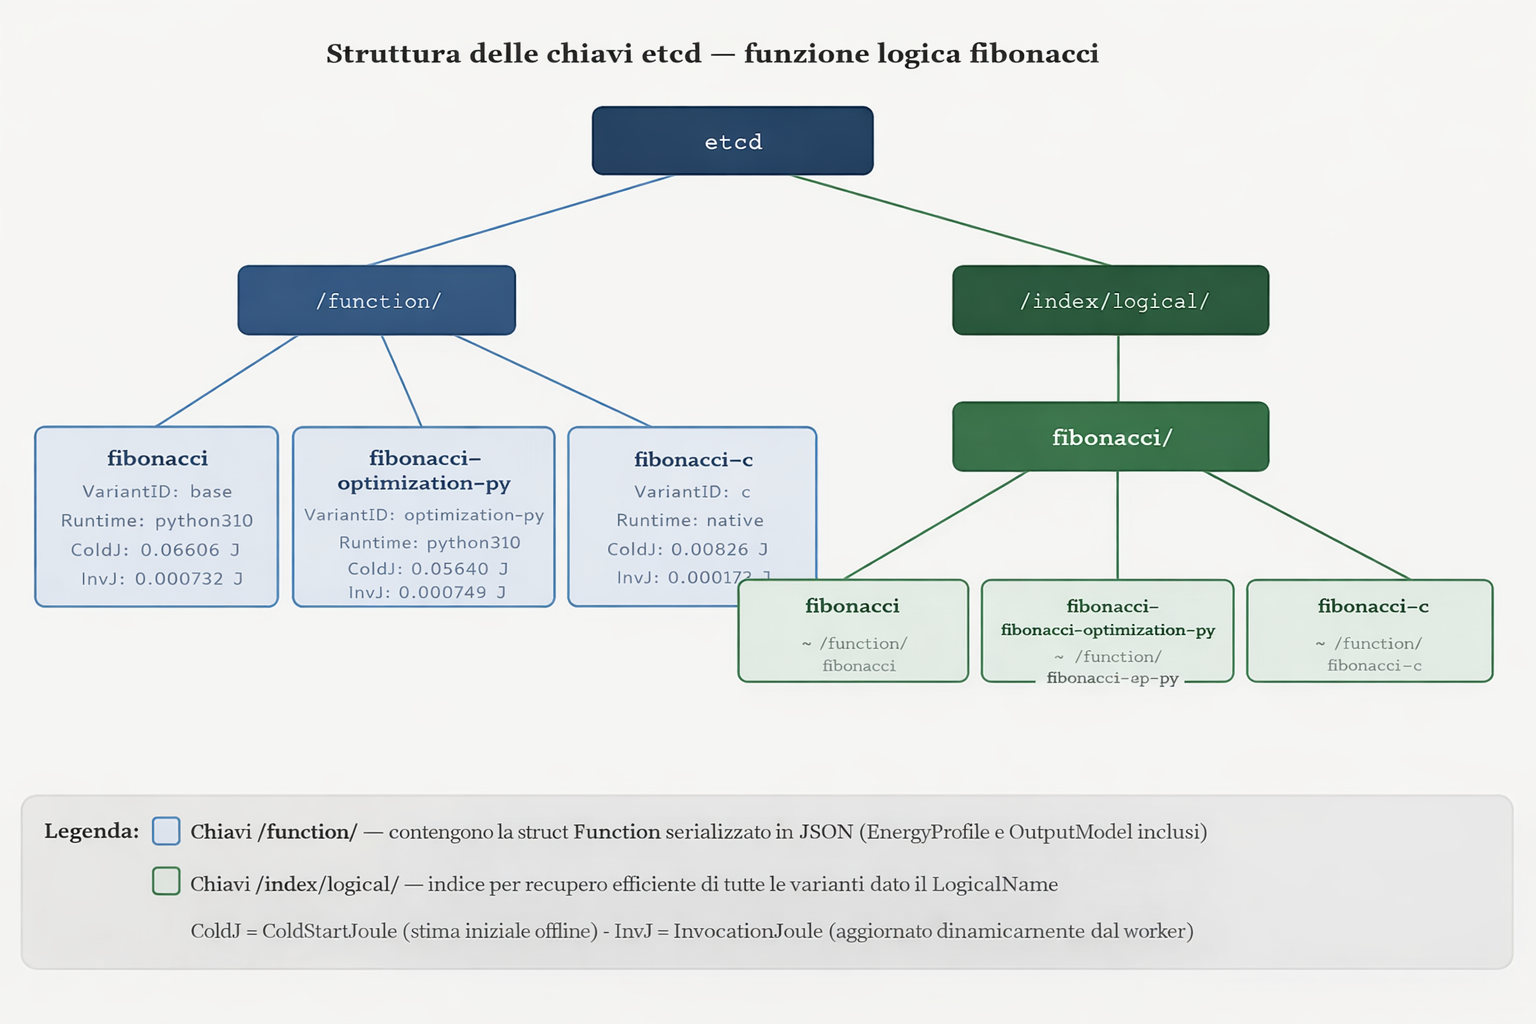
\includegraphics[width=0.95\textwidth]{figures/etcd-structure.jpg}
    \caption{Struttura delle chiavi etcd per la funzione logica 
    \texttt{fibonacci} con tre varianti. Le chiavi sotto 
    \texttt{/function/} contengono i profili completi aggiornati dal 
    worker periodico. L'indice sotto \texttt{/index/logical/} consente 
    allo scheduler di recuperare efficientemente le sole varianti della 
    funzione richiesta, senza scorrere l'intero store.}
    \label{fig:etcd-structure}
\end{figure}
%\section{Misurazione e aggiornamento adattivo dei profili energetici}
\label{sec:worker}

Una volta introdotto il modello di funzione logica con varianti multiple,
è necessario dotare il sistema di un meccanismo capace di aggiornare
dinamicamente i profili energetici sulla base dei consumi effettivamente
osservati a runtime. Un approccio statico, in cui il costo energetico di
una variante viene stimato offline e rimane invariato nel tempo, risulta
inadeguato in contesti di esecuzione reali: il consumo energetico di un
container è influenzato da fattori mutevoli quali il carico del nodo,
le interferenze tra istanze concorrenti e le variazioni dinamiche della
frequenza di CPU.

La soluzione adottata è un \emph{feedback loop} periodico che trasforma
il profilo energetico in una grandezza adattiva, aggiornata continuamente
in funzione del contesto di esecuzione. Il componente responsabile è un
worker di raccolta eseguito in background, illustrato in
Figura~\ref{fig:worker-architecture}.

\begin{figure}[ht]
    \centering
    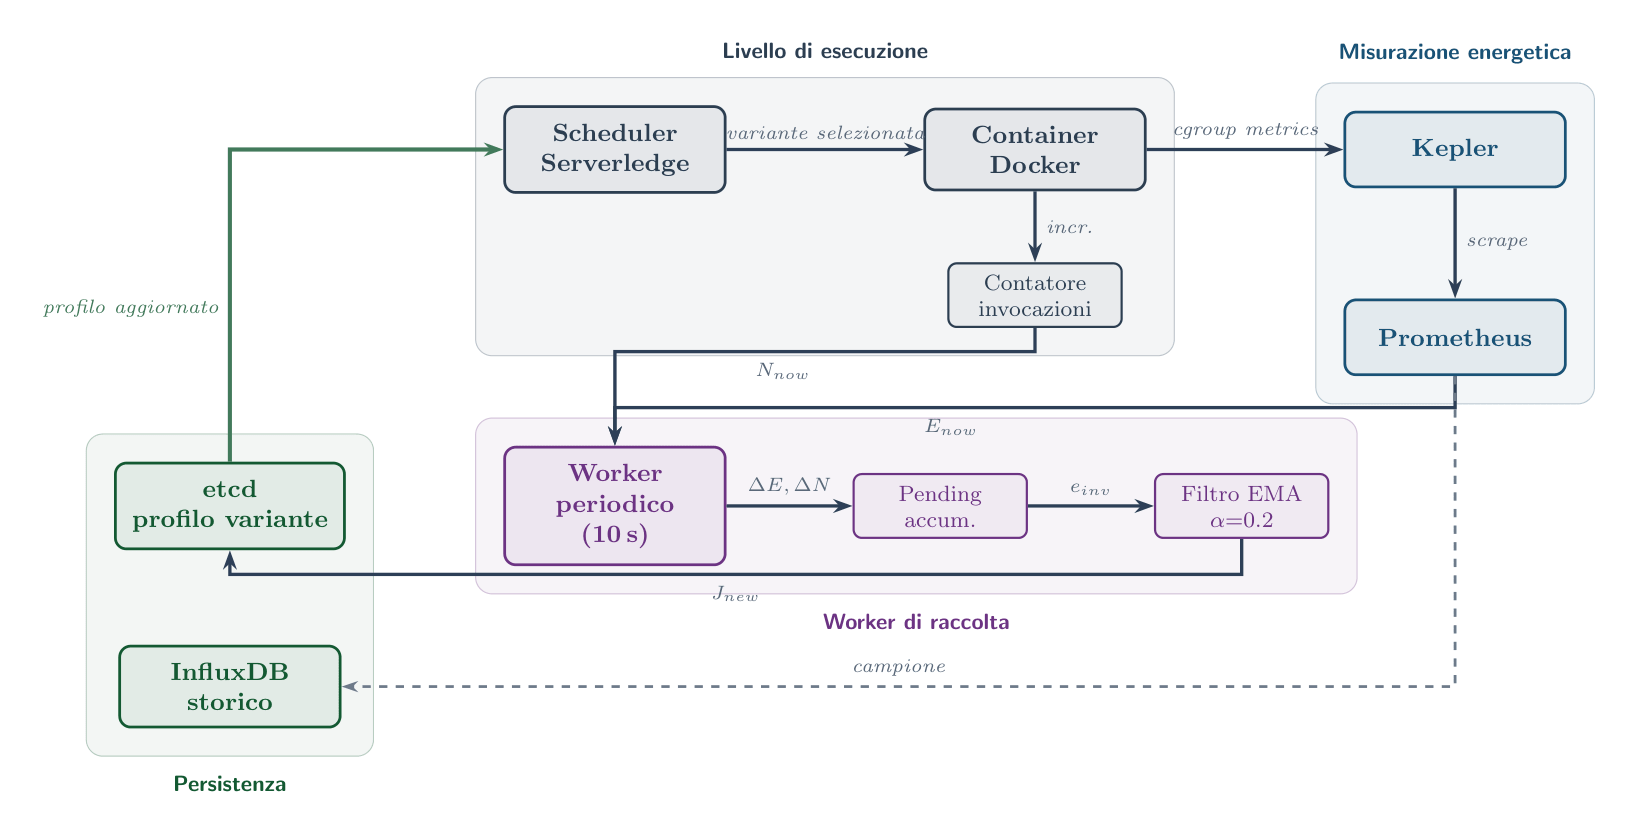
\includegraphics[width=\textwidth]{figures/Worker.png}
    \caption{Schema del feedback loop energetico. Il worker periodico
    legge le metriche cumulative da Kepler tramite Prometheus e il numero
    di invocazioni dal contatore locale, calcola i delta, applica un
    filtro EMA e aggiorna il profilo persistito in etcd, archiviando
    contestualmente i campioni in InfluxDB.}
    \label{fig:worker-architecture}
\end{figure}


\subsection{Tracciamento dei container e conteggio delle invocazioni}
\label{subsec:container-registry}

Per attribuire correttamente il consumo energetico alle singole varianti,
il sistema deve mantenere una corrispondenza stabile tra i container
Docker attivi e le funzioni in esecuzione. A tal fine il package
\texttt{energy} mantiene un registro in memoria che associa a ciascun
container una struttura \texttt{ContainerState} contenente:

\begin{itemize}
    \item l'identificatore del container (\texttt{ContainerID});
    \item il nome interno della variante (\texttt{FunctionName}), il
    \texttt{LogicalName} e il \texttt{VariantID};
    \item i valori di baseline dell'energia cumulativa e del numero di
    invocazioni (\texttt{LastJoule}, \texttt{LastInvocations}),
    impiegati per il calcolo dei delta incrementali;
    \item gli accumulatori \texttt{PendingEnergyJ} e
    \texttt{PendingInvocations}, necessari per gestire il disallineamento
    temporale tra metriche energetiche e contatori locali.
\end{itemize}

La registrazione avviene sia alla creazione del container sia, in modo
difensivo, al momento dell'invocazione, così da gestire correttamente il
caso di \emph{warm start}. Se un container è già presente nel registro,
la sua identità (mapping container-variante) non viene modificata,
garantendo coerenza per l'intero ciclo di vita del container.

Parallelamente, viene mantenuto un contatore atomico di invocazioni per
container, incrementato al completamento di ogni richiesta.

\subsection{Il worker periodico di raccolta}
\label{subsec:worker-periodico}

Il worker è implementato come una goroutine avviata all'inizializzazione
della piattaforma. Con cadenza di 10 secondi, esegue un ciclo di raccolta
(\texttt{Collect}) operando su uno snapshot thread-safe del
\texttt{ContainerRegistry}, in modo da isolare la lettura dallo stato
condiviso senza bloccare le operazioni concorrenti.

Per ciascun container attivo vengono acquisiti:

\begin{itemize}
    \item il valore cumulativo di energia $E_{now}$, esposto da Kepler e
    reso disponibile tramite l'endpoint Prometheus;
    \item il numero cumulativo di invocazioni $N_{now}$, mantenuto
    aggiornato dal contatore locale.
\end{itemize}

Vengono quindi calcolati i delta rispetto all'osservazione precedente:

\begin{equation}
    \Delta E = E_{now} - E_{last}
    \qquad
    \Delta N = N_{now} - N_{last}
\end{equation}

La presenza di valori negativi segnala un reset del container o del
contatore, condizione possibile ad esempio in seguito a un riavvio
dell'istanza, e comporta la reinizializzazione delle variabili senza
produzione di campioni, evitando attribuzioni energetiche errate.


\subsection{Attribuzione dell'energia per invocazione e gestione del lag}
\label{subsec:lag}

Le metriche esposte da Kepler hanno natura cumulativa e sono soggette a
un ritardo di campionamento intrinseco al ciclo di scraping di Prometheus.
Il contatore locale di invocazioni, al contrario, viene aggiornato
immediatamente al termine di ogni esecuzione. Può quindi verificarsi la
condizione:

\[
    \Delta N > 0 \quad \text{e} \quad \Delta E = 0
\]

in cui nuove invocazioni sono già state completate ma il relativo consumo
energetico non è ancora riflesso nella metrica cumulativa. Calcolare in
questo caso il consumo medio per invocazione produrrebbe una sottostima
sistematica.

Per gestire questo disallineamento, i delta vengono accumulati nei
campi \texttt{PendingEnergyJ} e \texttt{PendingInvocations}. L'attribuzione
effettiva avviene solo quando entrambi gli accumulatori risultano positivi,
garantendo che l'energia osservata e il numero di esecuzioni considerate
siano coerenti tra loro:

\begin{equation}
    e_{inv} = \frac{E_{pending}}{N_{pending}}
\end{equation}

Il valore $e_{inv}$ rappresenta la stima istantanea del consumo medio
per invocazione nel periodo considerato e costituisce l'ingresso per la
fase di aggiornamento adattivo del profilo.


\subsection{Aggiornamento del profilo tramite media mobile esponenziale}
\label{subsec:ema}

La stima istantanea $e_{inv}$ può essere affetta da rumore dovuto a
interferenze tra container, variazioni dinamiche della frequenza di CPU
o fluttuazioni del carico di sistema. Applicare direttamente tale valore
al profilo energetico potrebbe causare oscillazioni indesiderate nelle
decisioni dello scheduler.

Per stabilizzare la stima viene applicata una \emph{Exponential Moving
Average} (EMA):

\begin{equation}
    J_{new} = \alpha \cdot e_{inv} + (1 - \alpha) \cdot J_{old}
\end{equation}

con $\alpha = 0.2$. Il parametro $\alpha$ governa il compromesso tra
due esigenze contrastanti:

\begin{itemize}
    \item \textbf{Reattività}: valori elevati rendono il profilo
    rapidamente adattabile a variazioni strutturali del consumo energetico;
    \item \textbf{Stabilità}: valori ridotti attenuano il contributo
    di singoli campioni anomali, producendo una stima più robusta.
\end{itemize}

La scelta di $\alpha = 0.2$ rappresenta un equilibrio empirico: il
sistema filtra efficacemente i picchi transitori, mantenendo al
contempo una capacità di adattamento progressivo al nuovo regime
energetico nell'arco di circa $1/\alpha$ cicli di aggiornamento,
corrispondenti a circa 50 secondi con la cadenza attuale del worker.

Il valore aggiornato $J_{new}$ viene scritto nel campo
\texttt{InvocationJoule} della variante corrispondente e persistito in
etcd, rendendolo immediatamente disponibile allo scheduler per le
decisioni di selezione successive.



\subsection{Archiviazione su InfluxDB}
\label{subsec:influxdb}

Contestualmente all'aggiornamento in etcd, ogni campione viene archiviato
in InfluxDB come punto della \emph{measurement} \texttt{energy\_sample},
con tag \texttt{container\_id}, \texttt{logical\_name},
\texttt{function\_name}, \texttt{variant\_id} e campo
\texttt{invocation\_joule}.

La separazione tra i due store riflette le loro funzioni distinte: etcd
fornisce allo scheduler la stima corrente con latenza minima; InfluxDB
preserva la serie storica dei campioni, che costituisce la base
statistica per il meccanismo di esplorazione descritto nella
Sezione~\ref{sec:esplorazione-ucb}.

\section{Misurazione e aggiornamento adattivo dei profili energetici}
\label{sec:worker}

Una volta introdotto il modello di funzione logica con varianti multiple,
è necessario dotare il sistema di un meccanismo capace di aggiornare
dinamicamente i profili energetici sulla base dei consumi effettivamente
osservati a runtime. Un approccio statico, in cui il costo energetico di
una variante viene stimato offline e rimane invariato nel tempo, risulta
inadeguato in contesti di esecuzione reali: il consumo energetico di un
container è influenzato da fattori mutevoli quali il carico del nodo,
le interferenze tra istanze concorrenti e le variazioni dinamiche della
frequenza di CPU.

La soluzione adottata è un \emph{feedback loop} periodico che trasforma
il profilo energetico in una grandezza adattiva, aggiornata continuamente
in funzione del contesto di esecuzione. Il componente responsabile è un
worker di raccolta eseguito in background, illustrato in
Figura~\ref{fig:worker-architecture}.

\begin{figure}[ht]
    \centering
    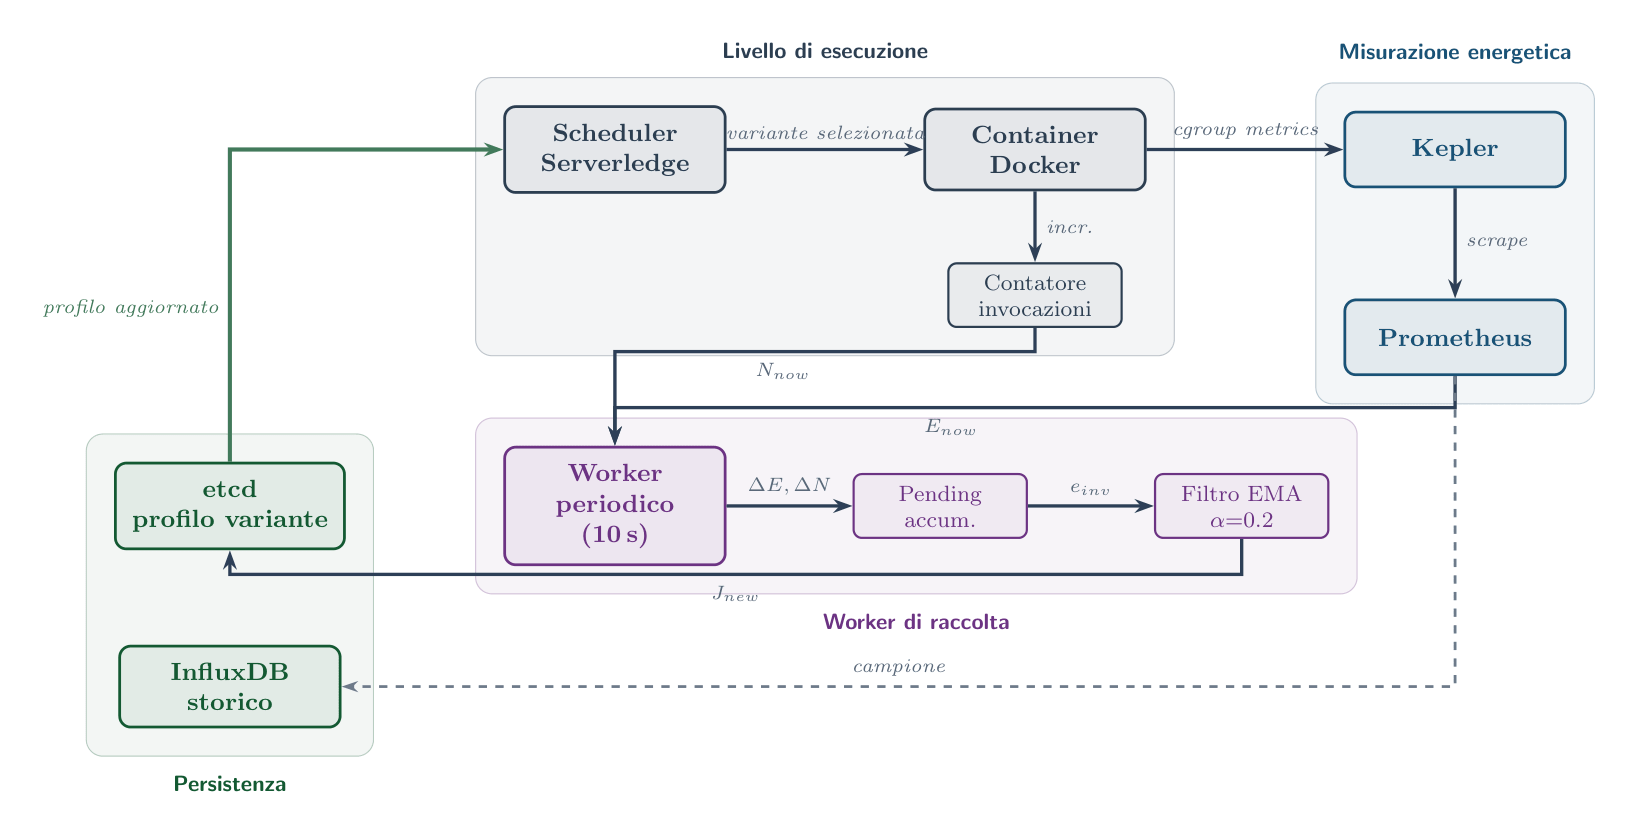
\includegraphics[width=\textwidth]{figures/Worker.png}
    \caption{Schema del feedback loop energetico. Il worker periodico
    legge le metriche cumulative da Kepler tramite Prometheus e il numero
    di invocazioni dal contatore locale, calcola i delta, applica un
    filtro EMA e aggiorna il profilo persistito in etcd, archiviando
    contestualmente i campioni in InfluxDB.}
    \label{fig:worker-architecture}
\end{figure}


\subsection{Tracciamento dei container e conteggio delle invocazioni}
\label{subsec:container-registry}

Per attribuire correttamente il consumo energetico alle singole varianti,
il sistema deve mantenere una corrispondenza stabile tra i container
Docker attivi e le funzioni in esecuzione. A tal fine il package
\texttt{energy} mantiene un registro in memoria che associa a ciascun
container una struttura \texttt{ContainerState} contenente:

\begin{itemize}
    \item l'identificatore del container (\texttt{ContainerID});
    \item il nome interno della variante (\texttt{FunctionName}), il
    \texttt{LogicalName} e il \texttt{VariantID};
    \item i valori di baseline dell'energia cumulativa e del numero di
    invocazioni (\texttt{LastJoule}, \texttt{LastInvocations}),
    impiegati per il calcolo dei delta incrementali;
    \item gli accumulatori \texttt{PendingEnergyJ} e
    \texttt{PendingInvocations}, necessari per gestire il disallineamento
    temporale tra metriche energetiche e contatori locali.
\end{itemize}

La registrazione avviene sia alla creazione del container sia, in modo
difensivo, al momento dell'invocazione, così da gestire correttamente il
caso di \emph{warm start}. Se un container è già presente nel registro,
la sua identità (mapping container-variante) non viene modificata,
garantendo coerenza per l'intero ciclo di vita del container.

Parallelamente, viene mantenuto un contatore atomico di invocazioni per
container, incrementato al completamento di ogni richiesta.

\subsection{Il worker periodico di raccolta}
\label{subsec:worker-periodico}

Il worker è implementato come una goroutine avviata all'inizializzazione
della piattaforma. Con cadenza di 10 secondi, esegue un ciclo di raccolta
(\texttt{Collect}) operando su uno snapshot thread-safe del
\texttt{ContainerRegistry}, in modo da isolare la lettura dallo stato
condiviso senza bloccare le operazioni concorrenti.

Per ciascun container attivo vengono acquisiti:

\begin{itemize}
    \item il valore cumulativo di energia $E_{now}$, esposto da Kepler e
    reso disponibile tramite l'endpoint Prometheus;
    \item il numero cumulativo di invocazioni $N_{now}$, mantenuto
    aggiornato dal contatore locale.
\end{itemize}

Vengono quindi calcolati i delta rispetto all'osservazione precedente:

\begin{equation}
    \Delta E = E_{now} - E_{last}
    \qquad
    \Delta N = N_{now} - N_{last}
\end{equation}

La presenza di valori negativi segnala un reset del container o del
contatore, condizione possibile ad esempio in seguito a un riavvio
dell'istanza, e comporta la reinizializzazione delle variabili senza
produzione di campioni, evitando attribuzioni energetiche errate.


\subsection{Attribuzione dell'energia per invocazione e gestione del lag}
\label{subsec:lag}

Le metriche esposte da Kepler hanno natura cumulativa e sono soggette a
un ritardo di campionamento intrinseco al ciclo di scraping di Prometheus.
Il contatore locale di invocazioni, al contrario, viene aggiornato
immediatamente al termine di ogni esecuzione. Può quindi verificarsi la
condizione:

\[
    \Delta N > 0 \quad \text{e} \quad \Delta E = 0
\]

in cui nuove invocazioni sono già state completate ma il relativo consumo
energetico non è ancora riflesso nella metrica cumulativa. Calcolare in
questo caso il consumo medio per invocazione produrrebbe una sottostima
sistematica.

Per gestire questo disallineamento, i delta vengono accumulati nei
campi \texttt{PendingEnergyJ} e \texttt{PendingInvocations}. L'attribuzione
effettiva avviene solo quando entrambi gli accumulatori risultano positivi,
garantendo che l'energia osservata e il numero di esecuzioni considerate
siano coerenti tra loro:

\begin{equation}
    e_{inv} = \frac{E_{pending}}{N_{pending}}
\end{equation}

Il valore $e_{inv}$ rappresenta la stima istantanea del consumo medio
per invocazione nel periodo considerato e costituisce l'ingresso per la
fase di aggiornamento adattivo del profilo.


\subsection{Aggiornamento del profilo tramite media mobile esponenziale}
\label{subsec:ema}

La stima istantanea $e_{inv}$ può essere affetta da rumore dovuto a
interferenze tra container, variazioni dinamiche della frequenza di CPU
o fluttuazioni del carico di sistema. Applicare direttamente tale valore
al profilo energetico potrebbe causare oscillazioni indesiderate nelle
decisioni dello scheduler.

Per stabilizzare la stima viene applicata una \emph{Exponential Moving
Average} (EMA):

\begin{equation}
    J_{new} = \alpha \cdot e_{inv} + (1 - \alpha) \cdot J_{old}
\end{equation}

con $\alpha = 0.2$. Il parametro $\alpha$ governa il compromesso tra
due esigenze contrastanti:

\begin{itemize}
    \item \textbf{Reattività}: valori elevati rendono il profilo
    rapidamente adattabile a variazioni strutturali del consumo energetico;
    \item \textbf{Stabilità}: valori ridotti attenuano il contributo
    di singoli campioni anomali, producendo una stima più robusta.
\end{itemize}

La scelta di $\alpha = 0.2$ rappresenta un equilibrio empirico: il
sistema filtra efficacemente i picchi transitori, mantenendo al
contempo una capacità di adattamento progressivo al nuovo regime
energetico nell'arco di circa $1/\alpha$ cicli di aggiornamento,
corrispondenti a circa 50 secondi con la cadenza attuale del worker.

Il valore aggiornato $J_{new}$ viene scritto nel campo
\texttt{InvocationJoule} della variante corrispondente e persistito in
etcd, rendendolo immediatamente disponibile allo scheduler per le
decisioni di selezione successive.



\subsection{Archiviazione su InfluxDB}
\label{subsec:influxdb}

Contestualmente all'aggiornamento in etcd, ogni campione viene archiviato
in InfluxDB come punto della \emph{measurement} \texttt{energy\_sample},
con tag \texttt{container\_id}, \texttt{logical\_name},
\texttt{function\_name}, \texttt{variant\_id} e campo
\texttt{invocation\_joule}.

La separazione tra i due store riflette le loro funzioni distinte: etcd
fornisce allo scheduler la stima corrente con latenza minima; InfluxDB
preserva la serie storica dei campioni, che costituisce la base
statistica per il meccanismo di esplorazione descritto nella
Sezione~\ref{sec:esplorazione-ucb}.
% ============================================================
%  Sezione 3.4 — Lo scheduler energy-aware
% ============================================================

\section{Lo scheduler energy-aware}
\label{sec:scheduler}

Lo scheduler energy-aware costituisce il componente decisionale centrale
dell'estensione progettata. Il suo compito è selezionare, tra le varianti
registrate per una data funzione logica, quella da eseguire concretamente
in risposta a ciascuna richiesta di invocazione. La selezione avviene
prima dell'assegnazione del container e dell'avvio dell'esecuzione vera e
propria, consentendo di sfruttare le stime energetiche aggiornate presenti
in \textit{etcd} come base per le proprie decisioni.

A differenza degli scheduler tradizionali, che operano esclusivamente a
livello di selezione del nodo di esecuzione, lo scheduler progettato
interviene a granularità di variante: a parità di funzione logica
richiesta, è possibile eseguire implementazioni alternative caratterizzate
da profili energetici e livelli di errore distinti. Questa scelta
progettuale consente di trattare il trade-off tra consumo energetico e
qualità del risultato come una grandezza controllabile a runtime, anziché
come una proprietà fissa dell'implementazione.

Il comportamento dello scheduler è ispirato ai meccanismi di controllo
runtime introdotti da JouleGuard~\cite{jouleguard}, adattati al paradigma
FaaS e al modello a varianti descritto nella Sezione~\ref{sec:variant-model}.
In particolare, il sistema non applica alcuna selezione alternativa in
assenza di un'esplicita autorizzazione da parte dell'utente, garantendo la
piena compatibilità con il comportamento legacy della piattaforma.

La logica decisionale dello scheduler si articola in tre casi distinti,
determinati dai parametri forniti dall'utente al momento dell'invocazione:
il caso base (senza abilitazione della variant selection), il caso di
selezione per errore minimo e il caso di selezione con vincolo
energetico esplicito. Tali casi sono analizzati nelle sezioni seguenti.

% --- FIGURA SUGGERITA -------------------------------------------
% Diagramma di flusso della logica decisionale dello scheduler:
% dall'invocazione in ingresso, biforcazione su AllowApprox,
% ramo error-first, ramo energy-budget, rifiuto HTTP 422.
%
% \begin{figure}[htbp]
%   \centering
%   \includegraphics[width=0.85\textwidth]{figures/scheduler_flow}
%   \caption{Flusso decisionale dello scheduler energy-aware. A seconda
%            del consenso fornito dall'utente e della presenza di un
%            vincolo energetico, il sistema applica politiche di selezione
%            distinte o preserva il comportamento legacy.}
%   \label{fig:scheduler_flow}
% \end{figure}
% ----------------------------------------------------------------


% ------------------------------------------------------------
\subsection{Il consenso esplicito dell'utente}
\label{sec:scheduler:consenso}
% ------------------------------------------------------------

Un principio fondamentale che guida la progettazione dello scheduler è la
separazione netta tra il comportamento di default della piattaforma e la
modalità energy-aware. La selezione di varianti alternative non viene attivata di default dalla piattaforma:
essa richiede sempre un consenso esplicito da parte dell'utente che
formula la richiesta di invocazione.

A tale scopo, l'interfaccia di invocazione è stata estesa con due campi
aggiuntivi: il flag booleano \texttt{AllowApprox} e il parametro
opzionale \texttt{MaxEnergyJoule}. Il primo esprime il consenso
dell'utente all'utilizzo di varianti alternative rispetto a quella
nominale; il secondo, se presente e positivo, specifica un budget
energetico massimo accettabile per l'invocazione, espresso in Joule.

In assenza di autorizzazione esplicita — ovvero quando
\texttt{AllowApprox = false} — la variant selection è completamente disabilitata e la
richiesta viene instradata verso la variante specificata nella chiamata,
secondo il comportamento originale della piattaforma. Questo garantisce la
piena compatibilità retroattiva con le applicazioni preesistenti e con gli
utenti che non desiderano delegare allo scheduler la scelta
dell'implementazione.

Quando invece \texttt{AllowApprox = true}, lo scheduler attiva la variant
selection energy-aware. In questo caso, tutte le varianti registrate per
la funzione logica corrispondente diventano candidate all'esecuzione e la
selezione avviene secondo criteri energetici e di errore,
eventualmente vincolati dal parametro \texttt{MaxEnergyJoule}. Il flusso
di controllo ad alto livello è formalizzato nell'Algoritmo~\ref{alg:submit}.

\begin{algorithm}[htbp]
\caption{\texttt{SubmitRequest} con variant selection opt-in}
\label{alg:submit}
\begin{algorithmic}[1]
\Function{SubmitRequest}{$r$ : \texttt{*function.Request}}
    \If{$r.\texttt{AllowApprox} = \textbf{true}$}
        \State $(\textit{selectedFn},\; \textit{err}) \gets
               \Call{SelectEnergyAwareVariant}{r}$
        \If{$\textit{err} \neq \textbf{nil}$}
            \State \Return $(\textbf{nil},\; \textit{err})$
            \Comment{vincolo energetico non soddisfatto → HTTP 422}
        \EndIf
        \If{$\textit{selectedFn} \neq \textbf{nil}$}
            \State $r.\texttt{Fun} \gets \textit{selectedFn}$
            \Comment{sostituisce la variante richiesta}
        \EndIf
    \EndIf
    \State $\textit{requests} \leftarrow r$
    \Comment{invia al loop legacy: \texttt{p.OnArrival(r)}}
    \State \Return \Call{SchedulingDecision}{$r$}
\EndFunction
\end{algorithmic}
\end{algorithm}

La struttura dell'algoritmo evidenzia come la variant selection si
inserisca come un livello di pre-elaborazione rispetto allo scheduler
originale: il risultato della selezione è la sostituzione della variante
richiesta con quella ottimale individuata dalla funzione
\textsc{SelectEnergyAwareVariant}, dopodiché l'esecuzione prosegue
secondo il percorso ordinario. In caso di errore — tipicamente quando
nessuna variante soddisfa i vincoli imposti — la richiesta viene rifiutata
con un codice di stato HTTP~422 (\textit{Unprocessable Entity}) senza
avviare alcuna computazione.


% ------------------------------------------------------------
\subsection{Selezione per errore minimo}
\label{sec:scheduler:error}
% ------------------------------------------------------------

Quando l'utente abilita la variant selection (\texttt{AllowApprox = true})
senza specificare un budget energetico, oppure con un valore
\texttt{MaxEnergyJoule} nullo o non positivo, lo scheduler opera secondo
la politica di \textit{accuracy-first}. In questo scenario, l'obiettivo è individuare la
variante che offre il risultato di qualità più elevata tra tutte quelle
disponibili, ricorrendo al consumo energetico stimato esclusivamente nel caso di parità di errore minimo tra due o più varianti.

La politica non applica alcun filtraggio energetico preventivo: tutte le
varianti registrate per la funzione logica sono candidate alla selezione,
indipendentemente dal loro profilo energetico. Questo approccio è coerente
con la natura opt-in del meccanismo: l'utente ha autorizzato l'uso di
varianti alternative, ma non ha imposto alcun vincolo sul consumo; la
piattaforma interpreta quindi tale consenso come un interesse prioritario
verso la qualità del risultato.

Per confrontare varianti con modelli di output eterogenei viene definita
una funzione di punteggio di errore $Err(v)$, costruita in modo tale
che valori numericamente inferiori corrispondano a errore minore.
La funzione è implementata nel componente \texttt{ErrorScore}$(v)$
secondo le regole seguenti:

\begin{itemize}
  \item se il modello di output della variante è di tipo \texttt{"error"},
        il punteggio è pari alla stima dell'errore associato:
        $Err(v) = \textit{ErrorEstimate}(v)$;

  \item se il modello è di tipo \texttt{"quality"}, la classe qualitativa
        viene convertita in una scala numerica ordinale:
        $\textit{High} \to 0$, $\textit{Medium} \to 1$, $\textit{Low} \to 2$;

  \item in assenza di un modello di output esplicito, si pone per
        convenzione $Err(v) = 0$, attribuendo l'errore minimo alla
        variante.
\end{itemize}

La selezione della variante ottimale $v^*$ avviene mediante
minimizzazione lessicografica sulla coppia $(Err(v),\, E(v))$, dove $E(v)$
rappresenta la stima energetica per l'invocazione:

\begin{equation}
  v^* = \arg\min_{v \in V}\; \bigl(Err(v),\; E(v)\bigr)
  \label{eq:error_first}
\end{equation}

In altri termini, tra tutte le varianti disponibili viene selezionata
quella con il punteggio di errore minore; in caso di parità, viene
preferita la variante con il consumo energetico stimato più basso. La
stima $E(v)$ è calcolata dalla funzione ausiliaria
\texttt{EnergyEstimate}$(v, \textit{warm})$, che distingue tra esecuzioni
a caldo (\textit{warm start}) e a freddo (\textit{cold start}):

\begin{equation}
  E(v) =
  \begin{cases}
    \textit{InvocationJoule}(v) & \text{se } \textit{isWarm} = \textbf{true} \\
    \textit{ColdStartJoule}(v) + \textit{InvocationJoule}(v)
      & \text{se } \textit{isWarm} = \textbf{false}
  \end{cases}
  \label{eq:energy_estimate}
\end{equation}

La determinazione dello stato warm viene effettuata dalla funzione
\texttt{WarmHint}$(v)$, che verifica l'esistenza di un container già
attivo utilizzabile per la variante $v$. In particolare, se la variante
espone il flag \texttt{ShareContainer = true}, il sistema considera warm
anche i container di altre varianti appartenenti alla stessa funzione
logica e con lo stesso runtime. Questo meccanismo di condivisione consente di
ridurre l'impatto del cold start nelle situazioni in cui una variante
priva di container attivo può beneficiare di un ambiente di esecuzione già
inizializzato da una variante affine.

I valori \textit{InvocationJoule} e \textit{ColdStartJoule} utilizzati
nella stima sono recuperati da \textit{etcd} al momento della selezione e
corrispondono all'ultima stima EMA disponibile per ciascuna variante,
aggiornata asincronamente dal worker di raccolta descritto nella
Sezione~\ref{sec:worker}. Lo scheduler opera quindi sempre sulla stima più
recente disponibile, con un ritardo rispetto al comportamento reale
dell'ordine di grandezza del periodo del worker.


% ------------------------------------------------------------
\subsection{Selezione con vincolo energetico}
\label{sec:scheduler:budget}
% ------------------------------------------------------------

Quando l'utente fornisce un budget energetico esplicito
(\texttt{MaxEnergyJoule} $> 0$), lo scheduler adotta la politica di
selezione con vincolo energetico, denominata \textit{energy-budget aware}.
In questa modalità il consumo energetico stimato diventa un vincolo
esplicito, e la minimizzazione dell'errore avviene all'interno
dell'insieme delle varianti compatibili con tale vincolo.

Il processo di selezione si articola nelle fasi descritte di seguito.

\medskip
\noindent\textbf{Fase 1 — Partizionamento delle varianti.}
Sia $B = \texttt{MaxEnergyJoule}$ il budget dichiarato dall'utente.
Tutte le varianti con stima energetica superiore a $B + \varepsilon$,
dove $\varepsilon = 0.05 \cdot B$, vengono scartate a priori.
Le rimanenti vengono ripartite in due insiemi disgiunti:

\begin{equation}
  F_{\text{strict}} = \{\, v : E(v) \leq B \,\}
  \label{eq:f_strict}
\end{equation}
\begin{equation}
  F_{\text{relaxed}} = \{\, v : B < E(v) \leq B + \varepsilon \,\}
  \label{eq:f_relaxed}
\end{equation}

$F_{\text{strict}}$ contiene le varianti che rispettano il budget in modo
esatto; $F_{\text{relaxed}}$ quelle che lo superano entro una fascia del
5\%, ammesse come zona di tolleranza. Se entrambi gli insiemi sono vuoti,
l'invocazione viene rifiutata con HTTP~422.

\medskip
\noindent\textbf{Fase 2 — Identificazione dei candidati finali.}
Da ciascun insieme viene estratta la variante con errore minimo:

\begin{align}
  v_1 &= \arg\min_{v \in F_{\text{strict}}}\; \bigl(\mathit{Err}(v),\; E(v)\bigr)
  \label{eq:v1} \\[4pt]
  v_2 &= \arg\min_{v \in F_{\text{relaxed}}}\; \bigl(\mathit{Err}(v),\; E(v)\bigr)
  \label{eq:v2}
\end{align}

dove $\mathit{Err}(v)$ è il punteggio di errore della variante, definito
nella Sezione~\ref{sec:scheduler:error}, e il consumo energetico agisce
solo a parità di errore. Se uno dei due insiemi è vuoto, il
candidato corrispondente non esiste e la selezione finale è immediata.

\medskip
\noindent\textbf{Fase 3 — Confronto e selezione finale.}
Quando entrambi i candidati esistono, si pone la domanda: conviene
sforare il budget scegliendo $v_2$? La risposta è affermativa solo se il
guadagno relativo in termini di riduzione dell'errore compensa proporzionalmente
lo sforamento relativo rispetto al budget. La condizione è:

\begin{equation}
  \frac{\mathit{Err}(v_1) - \mathit{Err}(v_2)}{\mathit{Err}(v_1)}
  \;>\;
  \frac{E(v_2) - B}{B}
  \label{eq:tradeoff}
\end{equation}

Il lato sinistro esprime la riduzione relativa dell'errore ottenuta
passando da $v_1$ a $v_2$, normalizzata rispetto all'errore di $v_1$
stesso — il punto di riferimento naturale, dato che è la migliore
alternativa entro vincolo. Il lato destro esprime la percentuale di
sforamento energetico rispetto al budget dichiarato, valore compreso per
costruzione nell'intervallo $(0,\, 0.05]$.
%L'interpretazione è diretta: se $v_2$ sfora il budget del 3\%, è
%accettabile solo se riduce l'errore di oltre il 3\% rispetto a $v_1$.
%Una riduzione inferiore non giustifica la violazione del vincolo.
Se la condizione~\eqref{eq:tradeoff} è soddisfatta, si sceglie $v_2$; altrimenti,
 si sceglie $v_1$.

Si osservi che, quando $\mathit{Err}(v_1) = 0$, la scelta fra $v_1$ e $v_2$ è banalmente $v_1$
dato che rispetta il vincolo ed ha errore minimo.

\medskip
\noindent\textbf{Fase 4 — Gestione del fallimento.}
Se entrambi gli insiemi $F_{\text{strict}}$ e $F_{\text{relaxed}}$ sono
vuoti — ovvero tutte le varianti superano $B + \varepsilon$ —
l'invocazione viene rifiutata con HTTP~422, senza eseguire alcuna
computazione.

La logica complessiva delle due politiche è formalizzata
nell'Algoritmo~\ref{alg:select}.\\
L'implementazione dell'algoritmo riflette la scelta di mantenere separata
la logica di selezione della variante dalla logica di assegnazione del
container e di esecuzione: \textsc{SelectEnergyAwareVariant} restituisce
esclusivamente la variante selezionata, lasciando invariato il percorso di
esecuzione successivo.

Complessivamente, lo scheduler energy-aware introduce un livello di controllo sul trade-off tra consumo energetico e qualità del risultato che opera esclusivamente su base consensuale, rispetta i profili energetici aggiornati a runtime e si integra con il meccanismo di condivisione dei container tra varianti. Il risultato è un sistema adattivo che, pur rimanendo trasparente agli utenti che non desiderano intervenire sulla selezione, è in grado di soddisfare vincoli energetici espliciti minimizzando l'errore del risultato compatibilmente con i vincoli imposti e, a parità di accuratezza, preferendo sempre la variante meno costosa energeticamente.

\begin{algorithm}[H]
\caption{\texttt{SelectEnergyAwareVariant}: politica a casi}
\label{alg:select}
\begin{algorithmic}[1]
\Function{SelectEnergyAwareVariant}{$r$ : \texttt{*function.Request}}
    \State $\textit{base} \gets r.\texttt{Fun}$
    \State $V \gets \Call{GetFunctionsByLogicalName}{\textit{base}.\texttt{LogicalName}}$
    \If{$V = \emptyset$}
        \State \Return $(\textit{base},\; \text{``fallback-base''},\; \textbf{nil})$
        \Comment{nessuna variante registrata}
    \EndIf
    \State $\textit{Eval} \gets [\,]$
    \For{$fn \in V$}
        \State $\textit{warm} \gets \Call{HasWarmContainer}{fn}$
        \State $E(fn) \gets \Call{energyCostJoule}{fn,\; \textit{warm}}$
        \State $\mathit{Err}(fn) \gets \Call{errorScore}{fn}$
        \State $\textit{Eval}.\textsc{Append}(fn,\; E(fn),\; \mathit{Err}(fn))$
    \EndFor
    \If{$r.\texttt{MaxEnergyJoule} = \textbf{nil}$ \textbf{or} $r.\texttt{MaxEnergyJoule} \leq 0$}
        \Comment{Case: error-first}
        \State $v^* \gets \arg\min_{\textit{Eval}} (\mathit{Err},\, E)$
        \State \Return $(v^*,\; \text{``error-first''},\; \textbf{nil})$
    \EndIf
    \State $B \gets r.\texttt{MaxEnergyJoule}$
    \Comment{Caso B: energy-budget}
    \State $\varepsilon \gets \Call{energyEpsilon}{B}$
    \Comment{$\varepsilon = 0.05 \cdot B$}
    \State $F_{\text{strict}}   \gets \{x \in \textit{Eval} \mid x.E \leq B\}$
    \State $F_{\text{relaxed}} \gets \{x \in \textit{Eval} \mid B < x.E \leq B + \varepsilon\}$
    \If{$F_{\text{strict}} = \emptyset$ \textbf{and} $F_{\text{relaxed}} = \emptyset$}
        \State \Return $(\textbf{nil},\; \text{``no-feasible-variants''},\; \textsc{Error})$
        \Comment{HTTP 422}
    \EndIf
    \If{$F_{\text{strict}} = \emptyset$}
        \State $v^* \gets \arg\min_{F_{\text{relaxed}}} (\mathit{Err},\, E)$
        \State \Return $(v^*,\; \text{``relaxed-only''},\; \textbf{nil})$
    \EndIf
    \If{$F_{\text{relaxed}} = \emptyset$}
        \State $v^* \gets \arg\min_{F_{\text{strict}}} (\mathit{Err},\, E)$
        \State \Return $(v^*,\; \text{``strict-only''},\; \textbf{nil})$
    \EndIf
    \State $v_1 \gets \arg\min_{F_{\text{strict}}} (\mathit{Err},\, E)$
    \State $v_2 \gets \arg\min_{F_{\text{relaxed}}} (\mathit{Err},\, E)$
    \If{$\dfrac{\mathit{Err}(v_1) - \mathit{Err}(v_2)}{\mathit{Err}(v_1)} \geq \dfrac{E(v_2) - B}{B}$}
        \State \Return $(v_2,\; \text{``relaxed-tradeoff''},\; \textbf{nil})$
    \Else
        \State \Return $(v_1,\; \text{``strict''},\; \textbf{nil})$
    \EndIf
\EndFunction
\end{algorithmic}
\end{algorithm}




\chapter{Risultati Sperimentali}
\label{cap:RisultatiSperimentali}
\include{src/capitoli/05-Conclusioni}
%==============Content===========================
\addcontentsline{toc}{chapter}{Elenco delle figure}
\listoffigures

\addcontentsline{toc}{chapter}{Elenco dei codici}
\lstlistoflistings

\addcontentsline{toc}{chapter}{Elenco degli algoritmi}
\listofalgorithms

% =====================================================
% BIBLIOGRAFIA
% =====================================================
\bibliographystyle{IEEEtran}
\bibliography{bibliografia/Bibliography}


\end{document}
